\chapter{Sprint 5 : Prédictions IA \& Chatbot Conversationnel}

\section*{Introduction}
\addcontentsline{toc}{section}{Introduction}
Le Sprint~5 complète Fleet~AI avec la couche d'Intelligence Artificielle. Six modèles de Machine Learning sont entraînés, évalués et déployés via une API FastAPI dédiée : scoring des chauffeurs, prévision de la demande par zone, détection des retards, dimensionnement de flotte, optimisation des tournées et évaluation du risque paiement. Chaque modèle suit la méthodologie CRISP-DM et est intégré directement dans l'interface métier concernée. En complément, un assistant conversationnel Text-to-SQL basé sur un LLM local (Gemma 4 31B via Ollama) permet aux managers d'interroger la base de données analytique en langage naturel, sans écrire de requêtes SQL. Ce sprint transforme Fleet~AI d'un outil de gestion en une plateforme décisionnelle intelligente.

\clearpage

% =============================================================
\section{Sprint Backlog}
% =============================================================

\textbf{Objectif du sprint :} L'objectif est de déployer la couche IA de Fleet~AI : six modèles prédictifs couvrant le scoring chauffeur, la demande, les retards, la flotte, les tournées et le risque paiement, ainsi qu'un assistant conversationnel Text-to-SQL accessible en langage naturel.

\definecolor{headerbg}{HTML}{d5f5e3}
\setlength{\arrayrulewidth}{1pt}

Les story points (SP) reflètent la complexité et l'effort de chaque tâche, estimés selon la suite de Fibonacci.

\begin{longtable}{|>{\raggedright\arraybackslash}p{4.2cm}|>{\raggedright\arraybackslash}p{4.8cm}|>{\raggedright\arraybackslash}p{4.5cm}|c|}
\hline
\rowcolor{headerbg}
\textbf{User Story} & \textbf{Tâche} & \textbf{Critères d'acceptation} & \textbf{\rotatebox{90}{SP}} \\
\hline
\endfirsthead
\hline
\rowcolor{headerbg}
\textbf{User Story} & \textbf{Tâche} & \textbf{Critères d'acceptation} & \textbf{\rotatebox{90}{SP}} \\
\hline
\endhead
\hline
\endfoot

%------ US-078 ------
\multirow{2}{=}{En tant que Planificateur, je veux des prédictions de la demande par zone et par jour dans mon tableau de bord afin d'anticiper les besoins en flotte.}
& Entraîner un modèle de prédiction de la demande à partir des données historiques de livraisons et le déployer dans le système. & Le modèle prédit la demande 7 jours à l'avance avec une précision jugée acceptable par l'équipe. & 8 \\
\cline{2-4}
& Afficher les prédictions de demande par zone et par jour dans le tableau de bord du Planificateur sous forme de graphique. & Les prédictions par zone et par jour sont affichées sous forme de graphique consultable. & 5 \\
\hline

%------ US-079 ------
\multirow{2}{=}{En tant que Planificateur, je veux des prédictions de retard pour chaque tournée dans mon tableau de bord afin d'agir préventivement.}
& Développer un modèle d'identification des tournées à risque de retard à partir des données historiques et des conditions opérationnelles. & Le modèle identifie les tournées à risque avec un taux de détection acceptable. & 5 \\
\cline{2-4}
& Afficher les tournées à risque avec un indicateur de confiance dans le tableau de bord du Planificateur. & Les tournées à risque sont mises en évidence avec un indicateur de niveau de risque (faible/moyen/élevé). & 3 \\
\hline

%------ US-080 ------
\multirow{2}{=}{En tant que Manager, je veux voir le niveau de confiance des prédictions dans mon tableau de bord afin de calibrer ma prise de décision.}
& Intégrer un indicateur de confiance à chaque prédiction exposée dans le tableau de bord Manager. & Chaque prédiction expose un niveau de confiance visible dans le tableau de bord. & 2 \\
\cline{2-4}
& Afficher l'indicateur de confiance par un repère visuel coloré sur chaque prédiction. & L'indicateur est visible sur chaque prédiction dans le tableau de bord. & 1 \\
\hline

%------ US-081 ------
\multirow{2}{=}{En tant qu'Administrateur, je veux que les modèles de prédiction soient réentraînés automatiquement périodiquement afin de maintenir leur précision.}
& Configurer un réentraînement automatique périodique des modèles de prédiction selon un calendrier défini. & Le réentraînement se déclenche automatiquement selon le calendrier configuré. & 3 \\
\cline{2-4}
& Alerter automatiquement le Manager si les indicateurs de performance des modèles se dégradent après réentraînement. & Une alerte est envoyée au Manager si la précision du modèle descend sous le seuil acceptable. & 2 \\
\hline

%------ US-082 ------
\multirow{2}{=}{En tant que Manager, je veux comparer les prédictions avec les réalisations dans mon tableau de bord afin d'évaluer la fiabilité du modèle.}
& Calculer et exposer au Manager l'écart entre les prédictions et les réalisations par zone et par semaine. & Le tableau comparatif affiche l'écart moyen par semaine et par zone. & 3 \\
\cline{2-4}
& Afficher la comparaison prédictions/réalisations avec filtres par période et par zone dans le tableau de bord. & Le graphique comparatif s'affiche avec filtres par période et par zone. & 2 \\
\hline

%------ US-083 ------
\multirow{2}{=}{En tant que Planificateur, je veux des recommandations pour le dimensionnement de la flotte dans mon tableau de bord afin d'optimiser le nombre de véhicules par zone.}
& Générer des recommandations de dimensionnement de flotte basées sur la demande prédite par zone. & Le système suggère le nombre optimal de véhicules par zone selon la demande prédite. & 3 \\
\cline{2-4}
& Afficher les recommandations de dimensionnement dans le tableau de bord avec comparaison face à la flotte actuelle. & Les recommandations sont affichées avec comparaison par rapport à la flotte existante. & 2 \\
\hline


%------ US-144 ------
\multirow{2}{=}{En tant que Manager, je veux interroger la base de données en langage naturel via un chatbot afin d'obtenir des analyses personnalisées.}
& Intégrer un modèle LLM local (Gemma) avec un pipeline Text-to-SQL pour traduire les questions en requêtes de base de données. & Le modèle génère des requêtes SQL valides correspondant aux intentions des utilisateurs. & 3 \\
\cline{2-4}
& Afficher l'interface de conversation dans l'application web avec historique des questions-réponses. & L'interface de chat est fonctionnelle ; l'historique est sauvegardé. & 2 \\
\hline

%------ US-145 ------
\multirow{2}{=}{En tant qu'Administrateur, je veux que le chatbot sécurise l'accès aux données selon le rôle de l'utilisateur afin de garantir la confidentialité.}
& Implémenter un validateur SQL (SQL Validator) pour bloquer les opérations d'écriture et vérifier les accès aux tables. & Le chatbot refuse toute requête DML ou DDL ; seules les tables autorisées sont interrogées. & 2 \\
\cline{2-4}
& Appliquer la sécurité au niveau des lignes (RLS) pour limiter les résultats au périmètre de l'utilisateur courant. & Les résultats sont filtrés selon le rôle (ex: le Manager ne voit que les stats de son périmètre). & 1 \\
\hline

\caption{Sprint Backlog du Sprint 5 --- Prédictions IA \& Chatbot Conversationnel}
\end{longtable}
\setlength{\arrayrulewidth}{0.4pt}


% =============================================================
\section{Modélisation IA selon la méthodologie CRISP-DM}
% =============================================================

Le sprint~5 introduit la couche prédictive de Fleet~AI : six modèles ML déployés via FastAPI, un chatbot Text-to-SQL sur LLM local, et un pipeline ETL industrialisé. La méthodologie \textbf{CRISP-DM} (\textit{Cross-Industry Standard Process for Data Mining}) cadre l'ensemble du cycle de vie, de la compréhension métier au déploiement en production.

% -----------------------------------------------------------
\subsection{Pipeline ETL -- Extraction, Transformation, Load}
% -----------------------------------------------------------

Avant tout entraînement, les données brutes issues du WFMS -- commandes ERP au format JSON, traces GPS, profils chauffeurs, historiques de paiement et logs d'audit -- doivent être préparées. Cette phase s'est révélée la difficulté centrale du sprint : la qualité des prédictions dépend directement de la rigueur du pipeline ETL.

% ============================================================
% FIGURE 8.1 — Pipeline ETL Fleet AI
% ============================================================
%
%  Layout (vertical, top-to-bottom) :
%
%   ┌─────────────────────────────────────────────────────────┐
%   │  Sources ERP / WFMS  (Ligne 0 — 5 nœuds gris)          │
%   │  S1   S2   S3   S4   S5                                 │
%   ├─────────────────────────────────────────────────────────┤
%   │  Étape 1 — Pré-traitement (Ligne 1 — 4 nœuds bleus)    │
%   │  E1 → E2 → E3 → E4                                     │
%   ├─────────────────────────────────────────────────────────┤
%   │  Étape 2 — Enrichissement (Ligne 2 — 4 nœuds)          │
%   │  E5 → E6 → E7(vert) → E8(bleu foncé)                   │
%   └─────────────────────────────────────────────────────────┘
%
%  Règles de routage sans croisement :
%  • S1→E1 : vertical direct
%  • S2,S3 → E2 : descendent à y=-1.4cm puis convergent vers E2
%  • S4,S5 → E4 : descendent à y=-1.4cm puis convergent vers E4
%  • E1→E5 : vertical direct (côté gauche)
%  • E4→E5 : passe en-dessous de la ligne 1 via y=-5.0cm
%             puis remonte à gauche (couloir x=-1.0cm) → E5
%  • E1→E2→E3→E4 : horizontaux directs
%  • E5→E6→E7→E8 : horizontaux directs
%
% ============================================================
% FIGURE 8.1 — Pipeline ETL Fleet AI
% ============================================================
\begin{figure}[H]
\centering
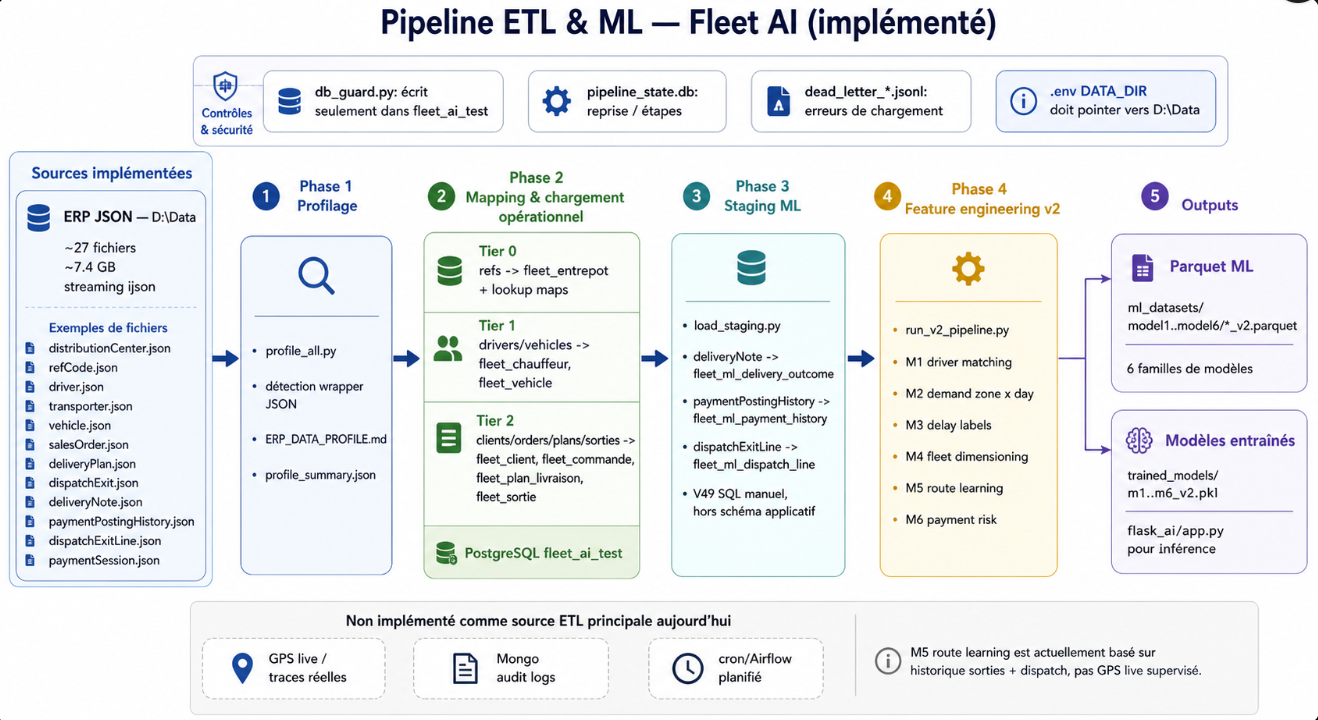
\includegraphics[width=\linewidth, keepaspectratio]{img/figure/ETL}
\caption{Pipeline ETL Fleet~AI --- Vue d'ensemble : de l'extraction ERP/WFMS à la sérialisation Parquet et au chargement PostgreSQL}
\label{fig:etl-pipeline}
\end{figure}



\subsubsection{Sources et extraction}

Le WFMS expose ses données sous forme de fichiers JSON hétérogènes dont la structure varie selon l'entité source (commandes, tournées, paiements, retours). Cinq catégories de sources sont ingérées :

\begin{itemize}
  \item fichiers de commandes ERP (champs manquants fréquents, encodages mixtes) ;
  \item traces GPS horodatées (intervalles irréguliers, coordonnées aberrantes) ;
  \item historiques de livraisons et statuts ;
  \item données client et transactions de paiement ;
  \item logs d'audit et événements métier.
\end{itemize}

\subsubsection{Transformation et nettoyage}

Le pipeline applique les transformations suivantes dans cet ordre :

\begin{enumerate}
  \item \textbf{Nettoyage} : suppression des doublons, correction des coordonnées GPS hors périmètre, normalisation des dates (ISO-8601).
  \item \textbf{Imputation} : valeurs manquantes imputées par médiane (variables continues) ou mode (variables catégorielles). Les colonnes dépassant 40\,\% de valeurs nulles sont exclues.
  \item \textbf{Résolution des incohérences} : détection par règles métier (ex. : livraison \texttt{LIVRÉE} sans horodatage, montant négatif) et mise en \textit{dead-letter queue} pour révision manuelle.
  \item \textbf{Normalisation} : variables numériques standardisées (StandardScaler) ; variables catégorielles encodées (One-Hot pour les zones géographiques, ordinal pour les niveaux de risque).
  \item \textbf{Feature engineering} : construction de variables métier dérivées -- taux de réussite historique par chauffeur, délai moyen de livraison par zone, charge hebdomadaire, score de ponctualité glissant sur 30~jours.
  \item \textbf{Agrégation temporelle} : fenêtres glissantes (1h, 24h, 7~jours) pour capturer les tendances de saisonnalité et les pics de demande.
\end{enumerate}

\subsubsection{Sérialisation et chargement}

Chaque modèle dispose d'un dataset dédié sérialisé au format \textbf{Parquet} (compression Snappy), choisi pour ses performances en lecture colonnaire et sa compatibilité native avec Pandas et PyArrow.

\begin{table}[H]
\centering
\setlength{\arrayrulewidth}{1pt}
\begin{tabular}{|l|l|r|}
\hline
\rowcolor{headerbg}
\textbf{Modèle} & \textbf{Dataset Parquet} & \textbf{Taille} \\
\hline
M1 -- Driver Scoring & \texttt{driver\_order\_pairs\_v2.parquet} & 11,5~Mo \\
\hline
M2 -- Demand Forecast & \texttt{demand\_features\_v2.parquet} & 2,3~Mo \\
\hline
M3 -- Delay Prediction & \texttt{delay\_features\_v2.parquet} & 8,9~Mo \\
\hline
M4 -- Fleet Dimensioning & \texttt{fleet\_features\_v2.parquet} & 1,6~Mo \\
\hline
M5 -- Route Learning & \texttt{route\_features\_v2.parquet} & 10,0~Mo \\
\hline
M6 -- Payment Risk & \texttt{payment\_risk\_v2.parquet} & 0,3~Mo \\
\hline
\end{tabular}
\caption{Datasets Parquet générés par le pipeline ETL}
\label{tab:datasets-parquet}
\end{table}
\setlength{\arrayrulewidth}{0.4pt}




% -----------------------------------------------------------
\subsection{M1 -- Driver Scoring : démarche CRISP-DM détaillée}
% -----------------------------------------------------------

Le modèle M1 constitue la référence pédagogique du sprint. Chaque phase CRISP-DM est détaillée ci-après.

\begin{figure}[H]
\centering
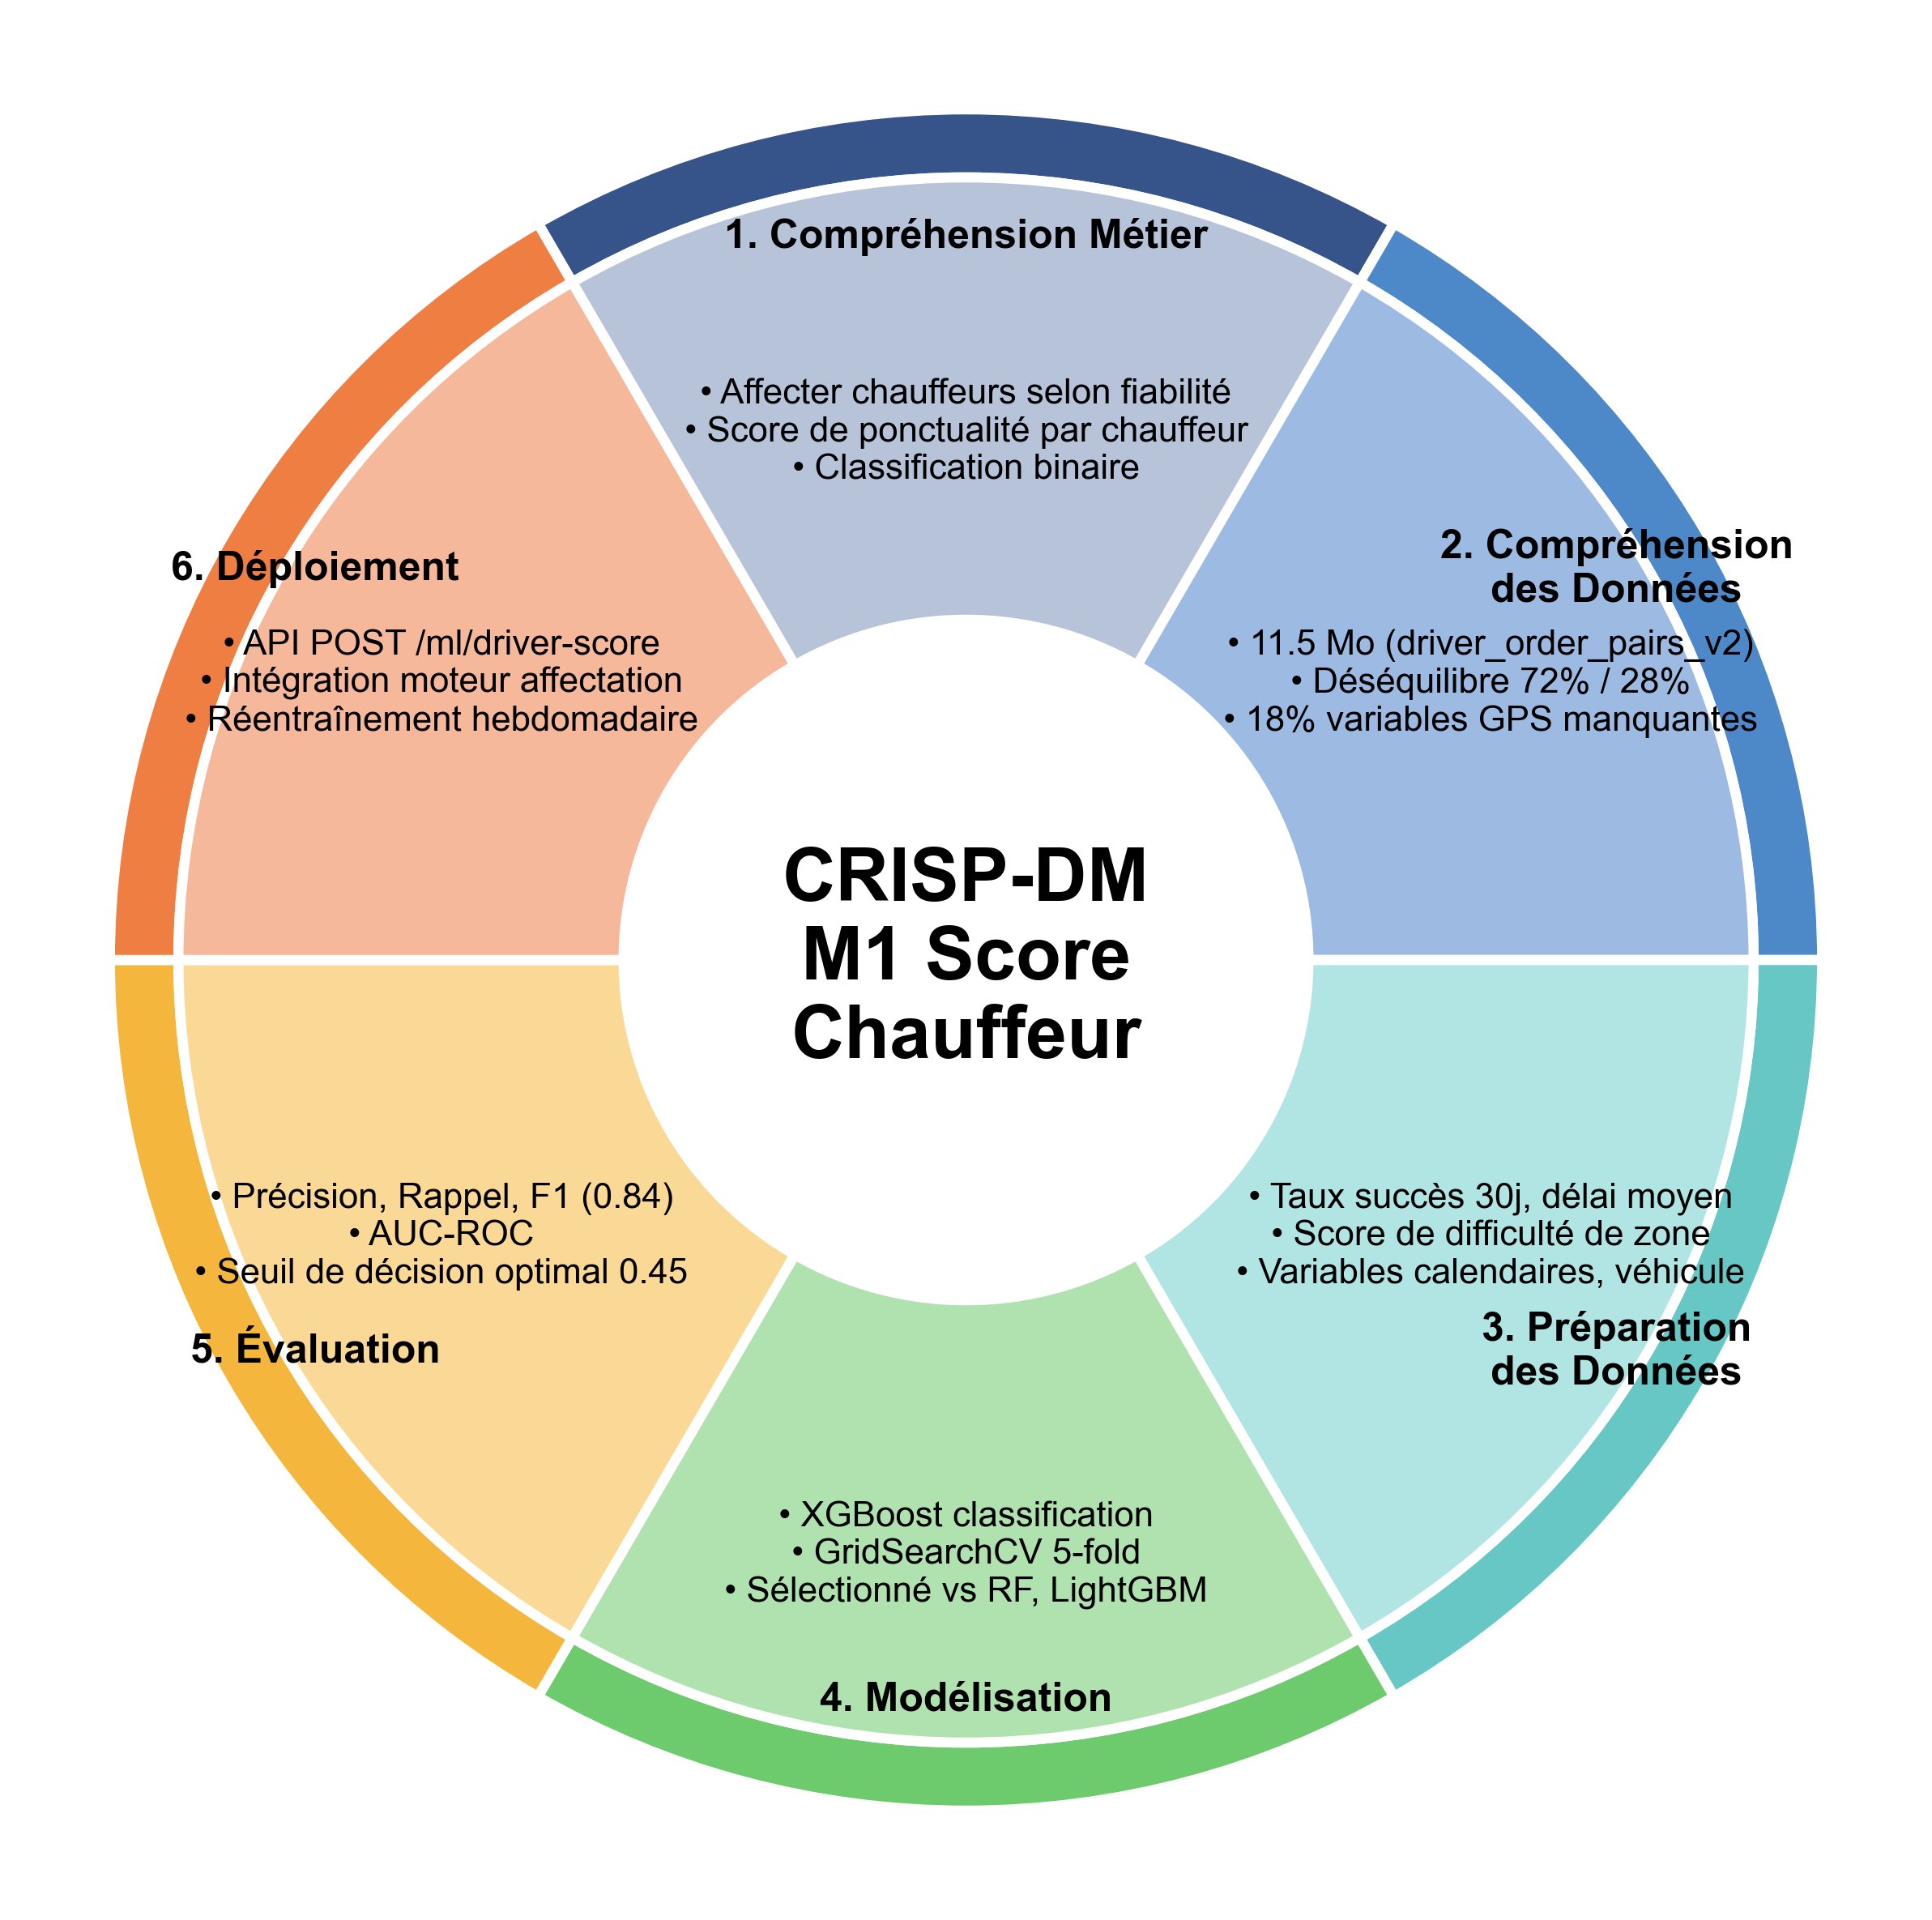
\includegraphics[width=0.90\linewidth]{img/crisp/crisp_dm_m1_driver}
\caption{Diagramme CRISP-DM -- M1 Score Chauffeur}
\label{fig:crisp-m1}
\end{figure}

\paragraph{Compréhension métier.}
Le planificateur de PGH doit affecter les chauffeurs aux tournées les plus adaptées à leur fiabilité. L'objectif est de produire un score de fiabilité par chauffeur, fondé sur son historique de ponctualité, afin d'alimenter le moteur d'affectation de Fleet~AI.

Problème modélisé : classification binaire de la ponctualité (\texttt{was\_on\_time} $\in \{0, 1\}$).

\paragraph{Compréhension des données.}
Dataset principal : \texttt{driver\_order\_pairs\_v2.parquet} (11,5~Mo, paires chauffeur--commande enrichies). Features initiales explorées : profil du chauffeur (ancienneté, type de permis), zone de livraison, tranche horaire, conditions de la tournée, historique de 90~jours.

Principaux constats d'exploration :
\begin{itemize}
  \item distribution déséquilibrée (72\,\% on-time / 28\,\% retard) ;
  \item forte corrélation entre zone et taux de retard ;
  \item variables GPS manquantes à 18\,\% -- gérées nativement par XGBoost.
\end{itemize}

\paragraph{Préparation des données.}
Application du pipeline ETL (\S~8.2.1). Features retenues après sélection :

\begin{itemize}
  \item \texttt{driver\_success\_rate\_30d} -- taux de réussite glissant 30~jours ;
  \item \texttt{avg\_delivery\_delay\_min} -- délai moyen historique en minutes ;
  \item \texttt{zone\_difficulty\_score} -- score de complexité de la zone ;
  \item \texttt{order\_count\_day} -- charge journalière du chauffeur ;
  \item \texttt{hour\_of\_day}, \texttt{day\_of\_week} -- variables calendaires ;
  \item \texttt{vehicle\_type\_encoded} -- type de véhicule (One-Hot).
\end{itemize}

\paragraph{Modélisation et justification du modèle.}
Cinq algorithmes ont été évalués lors de cette phase : Régression Logistique, Réseau de Neurones (MLP), Random Forest, LightGBM et XGBoost. Les résultats obtenus sur un jeu de test (20\,\% des données) sont présentés dans le tableau~\ref{tab:m1-evaluation}.

\begin{table}[H]
\centering
\setlength{\arrayrulewidth}{1pt}
\begin{tabular}{|l|c|c|p{4cm}|}
\hline
\rowcolor{headerbg}
\textbf{Algorithme} & \textbf{Précision (Accuracy)} & \textbf{F1-Score} & \textbf{Temps d'entraînement} \\
\hline
Régression Logistique & 68,5\,\% & 0,62 & Très rapide (< 10 s) \\
\hline
Réseau de Neurones (MLP) & 74,2\,\% & 0,71 & Lent ($\approx$ 12 min) \\
\hline
Random Forest & 81,4\,\% & 0,78 & Moyen ($\approx$ 3 min) \\
\hline
LightGBM & 83,1\,\% & 0,81 & Très rapide ($\approx$ 15 s) \\
\hline
\textbf{XGBoost} & \textbf{85,7\,\%} & \textbf{0,84} & \textbf{Rapide ($\approx$ 30 s)} \\
\hline
\end{tabular}
\caption{Comparatif des algorithmes évalués pour le modèle M1}
\label{tab:m1-evaluation}
\end{table}
\setlength{\arrayrulewidth}{0.4pt}

L'algorithme \textbf{XGBoost} a été retenu. En plus de fournir les meilleures performances (F1-Score de 0,84), il gère nativement les valeurs manquantes (fréquentes avec les signaux GPS), résiste bien au surapprentissage grâce à sa régularisation (L1/L2), et offre une grande interprétabilité (importance des features) cruciale pour expliquer les scores aux planificateurs.

Un classificateur XGBoost a donc été entraîné avec une recherche sur grille (\textit{GridSearchCV}, 5-fold stratifié) sur les hyperparamètres : \texttt{max\_depth} $\in$ \{4, 6, 8\}, \texttt{learning\_rate} $\in$ \{0.05, 0.1\}, \texttt{n\_estimators} $\in$ \{200, 400\}. Le paramètre \texttt{scale\_pos\_weight} compense le déséquilibre de classes.

\paragraph{Évaluation.}
Métriques retenues : Précision, Rappel, F1-Score et AUC-ROC. La matrice de confusion valide le seuil de décision optimal à 0.45 (maximisation du F1 sur la classe minoritaire).

\paragraph{Déploiement.}
Le modèle sérialisé (\texttt{joblib}) est exposé via une route FastAPI \texttt{POST /api/v1/ml/driver-score}. Le score retourné (0--100) est intégré directement dans l'algorithme d'affectation de Fleet~AI. Un réentraînement automatique est planifié hebdomadairement.

\paragraph{Intégration dans l'application.}
Le score du modèle M1 est visible par le Planificateur dans le formulaire d'affectation~: les trois meilleurs candidats chauffeurs sont classés par score de fiabilité (0--100), avec la décomposition des critères (zone, charge, performance). Ce score alimente également le module de suggestions du Sprint~5.

\begin{figure}[H]
\centering
\IfFileExists{img/capture/ai/sp5_m1_driver_score_composite.png}{%
  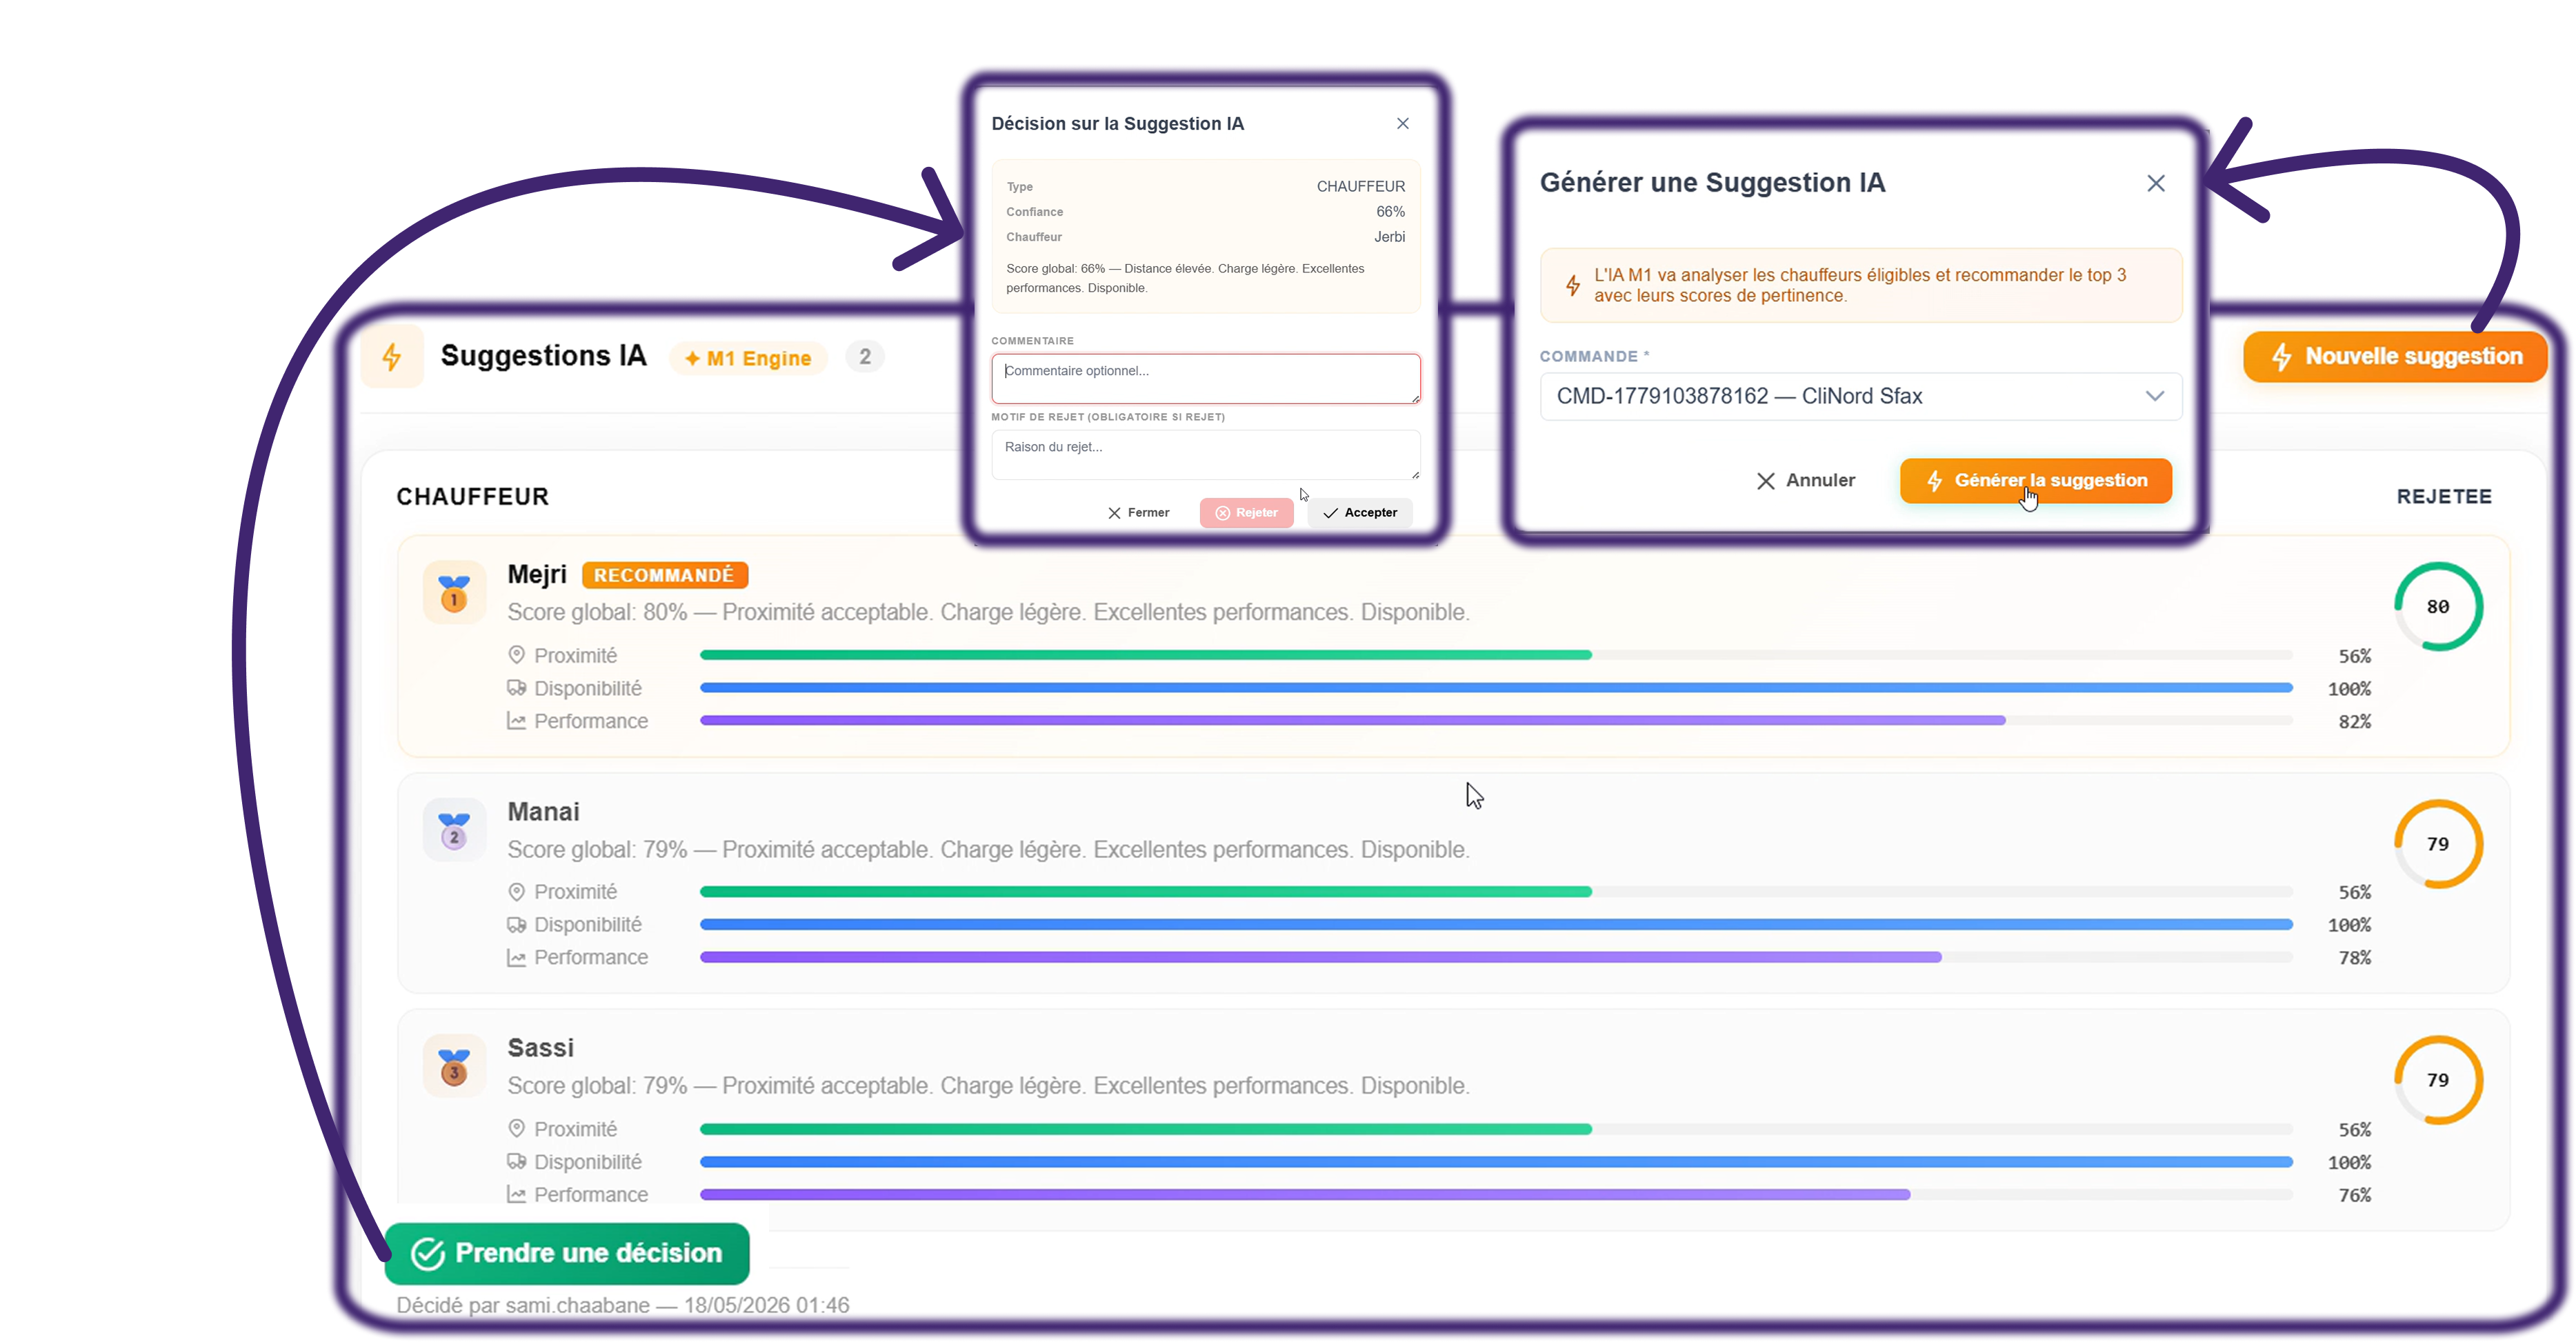
\includegraphics[width=\linewidth, keepaspectratio]{img/capture/ai/sp5_m1_driver_score_composite}%
}{%
  \fbox{\parbox{0.9\linewidth}{\centering\vspace{4cm}\textit{[\`{}img/sp5\_m1\_driver\_score\_composite\`{} --- Capture à réaliser]}\vspace{4cm}}}%
}
\caption{Intégration M1 Driver Scoring : formulaire d'affectation avec scores de fiabilité, top~3 chauffeurs et décomposition des critères}
\label{fig:sp5-m1-integration}
\end{figure}

% -----------------------------------------------------------
\subsection{Modèles prédictifs additionnels (M2 à M6)}
% -----------------------------------------------------------

Les modèles M2 à M6 suivent la même méthodologie CRISP-DM. Pour chacun de ces modèles, l'algorithme XGBoost a été retenu pour les mêmes raisons de performance, de gestion des données tabulaires et de robustesse que celles justifiées lors de la modélisation de M1. Seuls les éléments distinctifs de chaque modèle sont présentés ci-après.

\subsubsection{M2 -- Demand Forecast}

\begin{figure}[H]
\centering
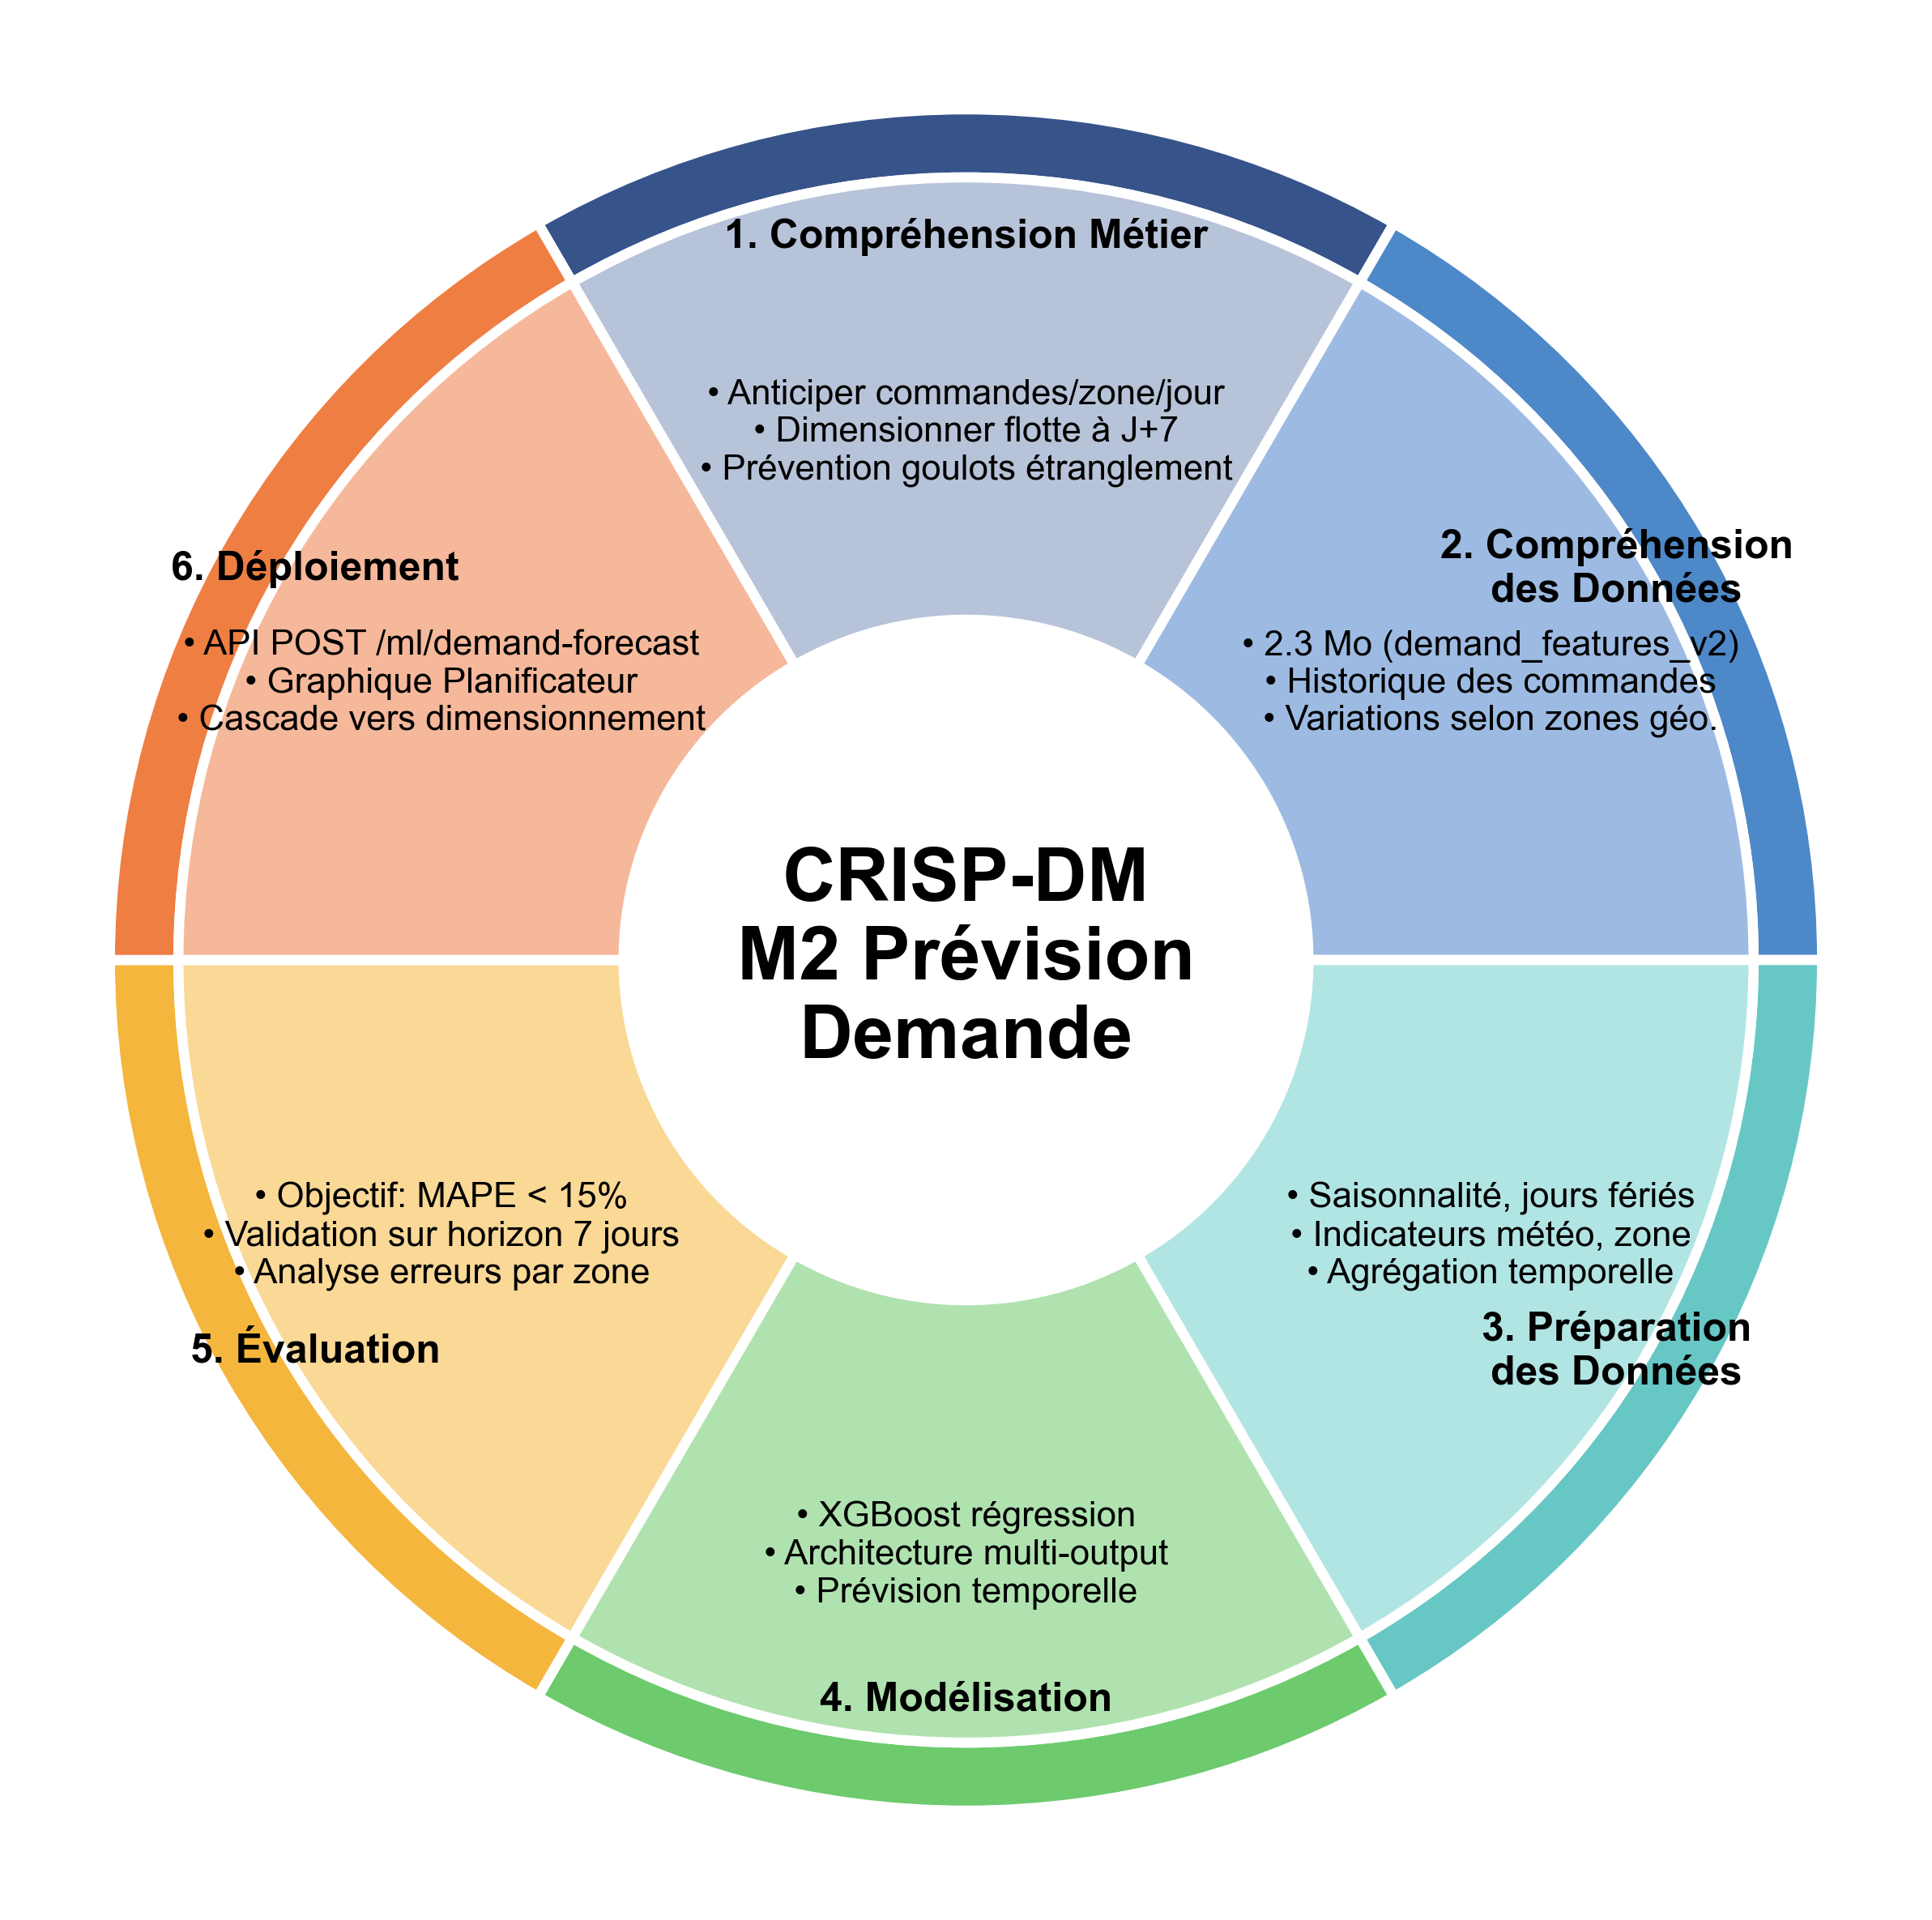
\includegraphics[width=0.88\linewidth]{img/crisp/crisp_dm_m2_demand}
\caption{Diagramme CRISP-DM -- M2 Prévision de la Demande}
\label{fig:crisp-m2}
\end{figure}

\begin{table}[H]
\centering
\setlength{\arrayrulewidth}{1pt}
\begin{tabular}{|p{3.5cm}|p{9.5cm}|}
\hline
\rowcolor{headerbg}
\multicolumn{2}{|c|}{\textbf{M2 -- Demand Forecast}} \\
\hline
\textbf{Objectif métier} & Anticiper le volume de commandes par zone et par jour pour dimensionner la flotte à J+7. \\
\hline
\textbf{Dataset} & \texttt{demand\_features\_v2.parquet} (2,3~Mo) \\
\hline
\textbf{Features clés} & Historique de commandes, saisonnalité, jours fériés, zone géographique, indicateurs météo. \\
\hline
\textbf{Algorithme} & XGBoost régression multi-output (une sortie par zone). \\
\hline
\textbf{Métrique cible} & MAPE $<$ 15\,\% sur l'horizon 7~jours. \\
\hline
\textbf{Intégration} & Tableau de bord Planificateur -- graphique de prévision par zone. \\
\hline
\end{tabular}
\caption{Fiche synthétique -- M2 Demand Forecast}
\label{tab:m2-summary}
\end{table}
\setlength{\arrayrulewidth}{0.4pt}

\paragraph{Intégration dans l'application.}
Les prévisions de la demande par zone et par jour sont affichées sous forme de graphique interactif dans le tableau de bord du Planificateur. L'horizon est de 7~jours avec un indicateur de fiabilité (MAPE).

\begin{figure}[H]
\centering
\IfFileExists{img/capture/ai/sp5_m2_demand_forecast_composite.png}{%
  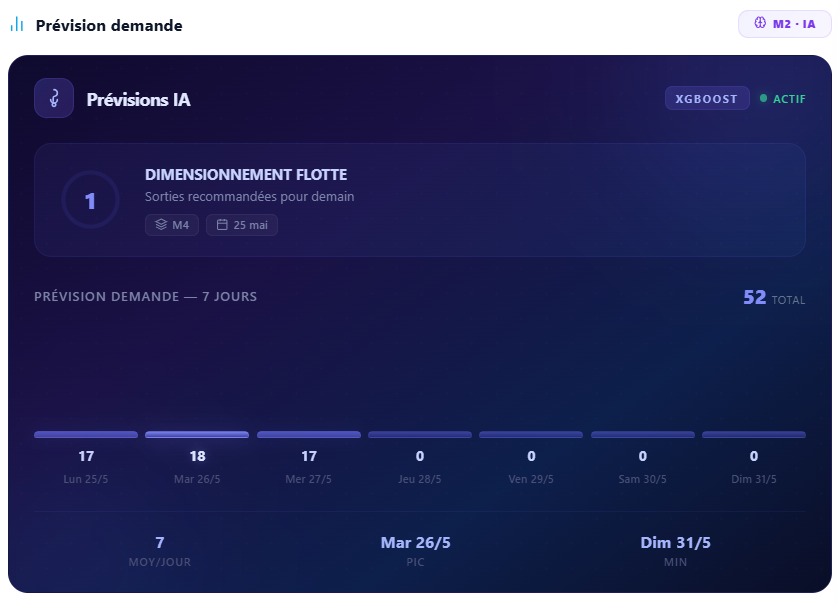
\includegraphics[width=\linewidth, keepaspectratio]{img/capture/ai/sp5_m2_demand_forecast_composite}%
}{%
  \fbox{\parbox{0.9\linewidth}{\centering\vspace{4cm}\textit{[\`{}img/sp5\_m2\_demand\_forecast\_composite\`{} --- Capture à réaliser]}\vspace{4cm}}}%
}
\caption{Intégration M2 Demand Forecast : tableau de bord Planificateur avec graphique de prévision de la demande par zone sur 7~jours}
\label{fig:sp5-m2-integration}
\end{figure}

\subsubsection{M3 -- Delay Prediction}

\begin{figure}[H]
\centering
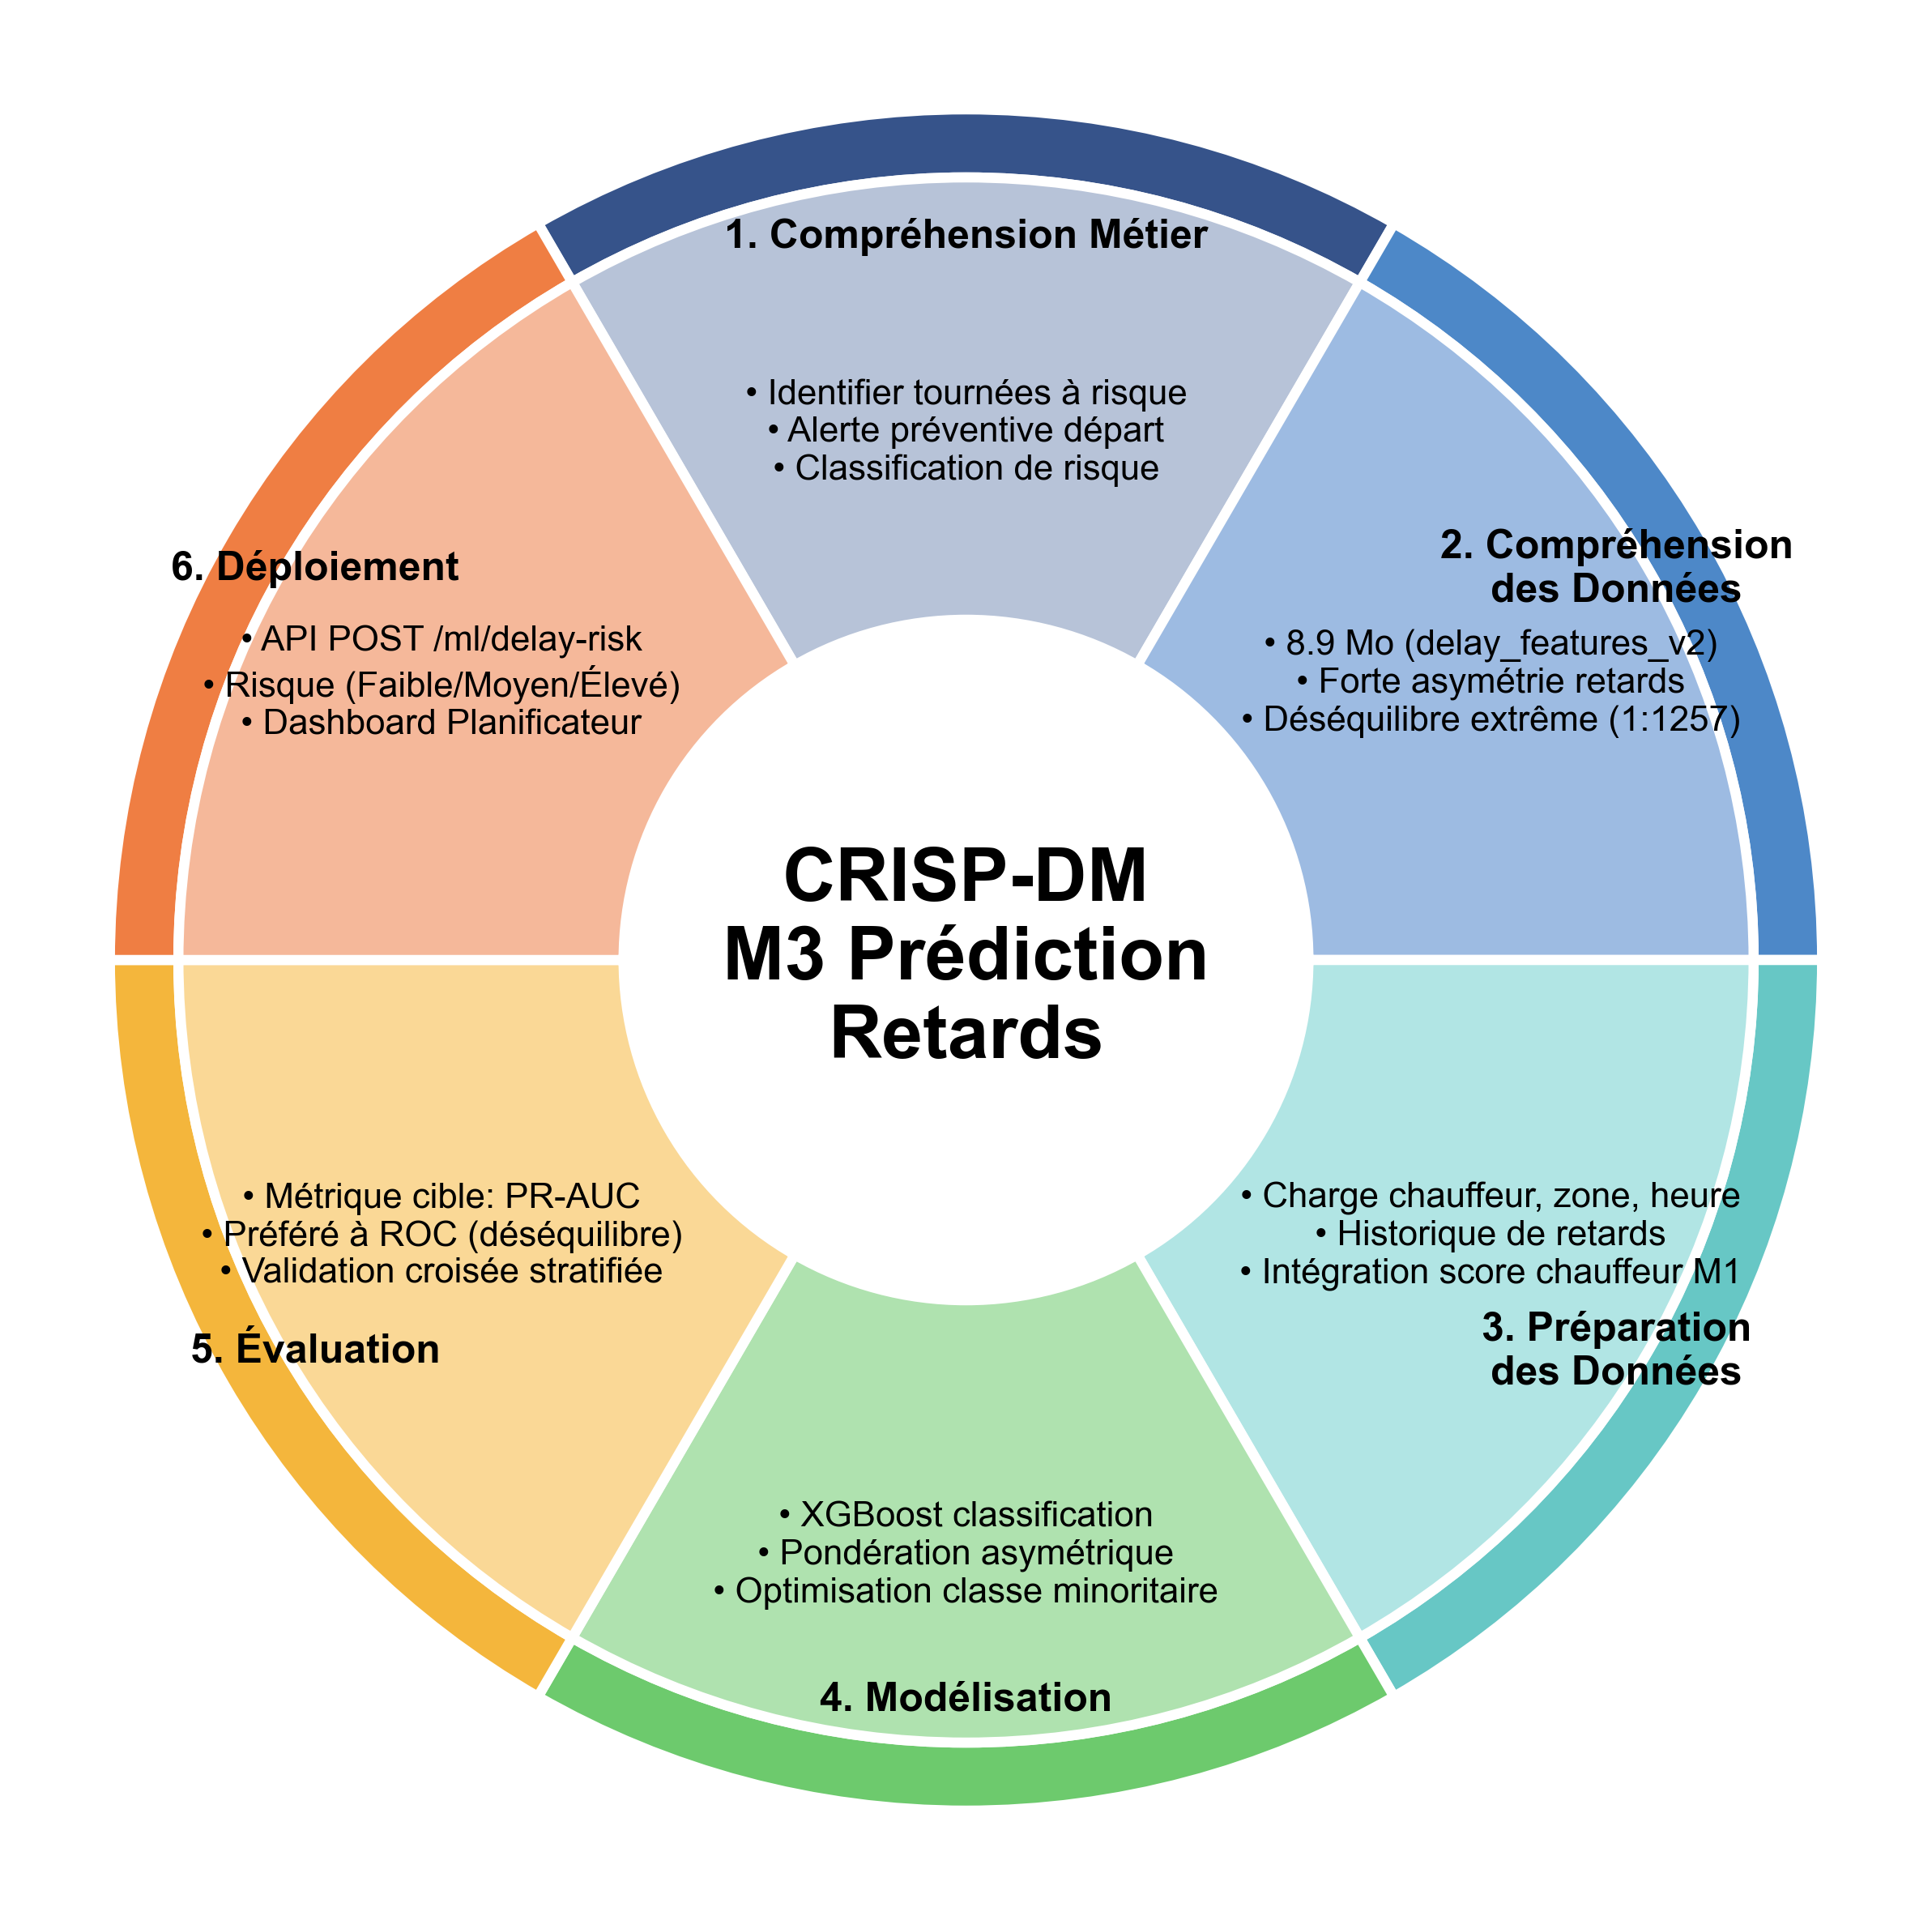
\includegraphics[width=0.88\linewidth]{img/crisp/crisp_dm_m3_delay}
\caption{Diagramme CRISP-DM -- M3 Prédiction des Retards}
\label{fig:crisp-m3}
\end{figure}

\begin{table}[H]
\centering
\setlength{\arrayrulewidth}{1pt}
\begin{tabular}{|p{3.5cm}|p{9.5cm}|}
\hline
\rowcolor{headerbg}
\multicolumn{2}{|c|}{\textbf{M3 -- Delay Prediction}} \\
\hline
\textbf{Objectif métier} & Identifier les tournées à risque de retard avant leur départ pour intervention préventive. \\
\hline
\textbf{Dataset} & \texttt{delay\_features\_v2.parquet} (8,9~Mo) \\
\hline
\textbf{Features clés} & Charge du chauffeur, zone, heure de départ, historique de retards, score M1. \\
\hline
\textbf{Algorithme} & XGBoost classification, pondération asymétrique des coûts (déséquilibre 1:1257). \\
\hline
\textbf{Métrique cible} & PR-AUC (plus représentative que ROC sur classes déséquilibrées). \\
\hline
\textbf{Intégration} & Indicateur de risque (Faible / Moyen / Élevé) dans le tableau de bord Planificateur. \\
\hline
\end{tabular}
\caption{Fiche synthétique -- M3 Delay Prediction}
\label{tab:m3-summary}
\end{table}
\setlength{\arrayrulewidth}{0.4pt}

\paragraph{Intégration dans l'application.}
L'indicateur de risque de retard (Faible~/ Moyen~/ Élevé) est affiché en couleur sur chaque tournée du tableau de bord Planificateur, permettant une intervention préventive avant le départ.

\begin{figure}[H]
\centering
\IfFileExists{img/capture/ai/sp5_m3_delay_prediction_composite.png}{%
  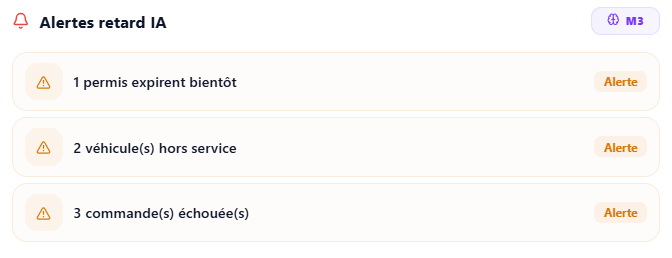
\includegraphics[width=\linewidth, keepaspectratio]{img/capture/ai/sp5_m3_delay_prediction_composite}%
}{%
  \fbox{\parbox{0.9\linewidth}{\centering\vspace{4cm}\textit{[\`{}img/sp5\_m3\_delay\_prediction\_composite\`{} --- Capture à réaliser]}\vspace{4cm}}}%
}
\caption{Intégration M3 Delay Prediction : indicateur de risque de retard (Faible / Moyen / Élevé) dans le tableau de bord Planificateur}
\label{fig:sp5-m3-integration}
\end{figure}

\subsubsection{M4 -- Fleet Dimensioning}

\begin{figure}[H]
\centering
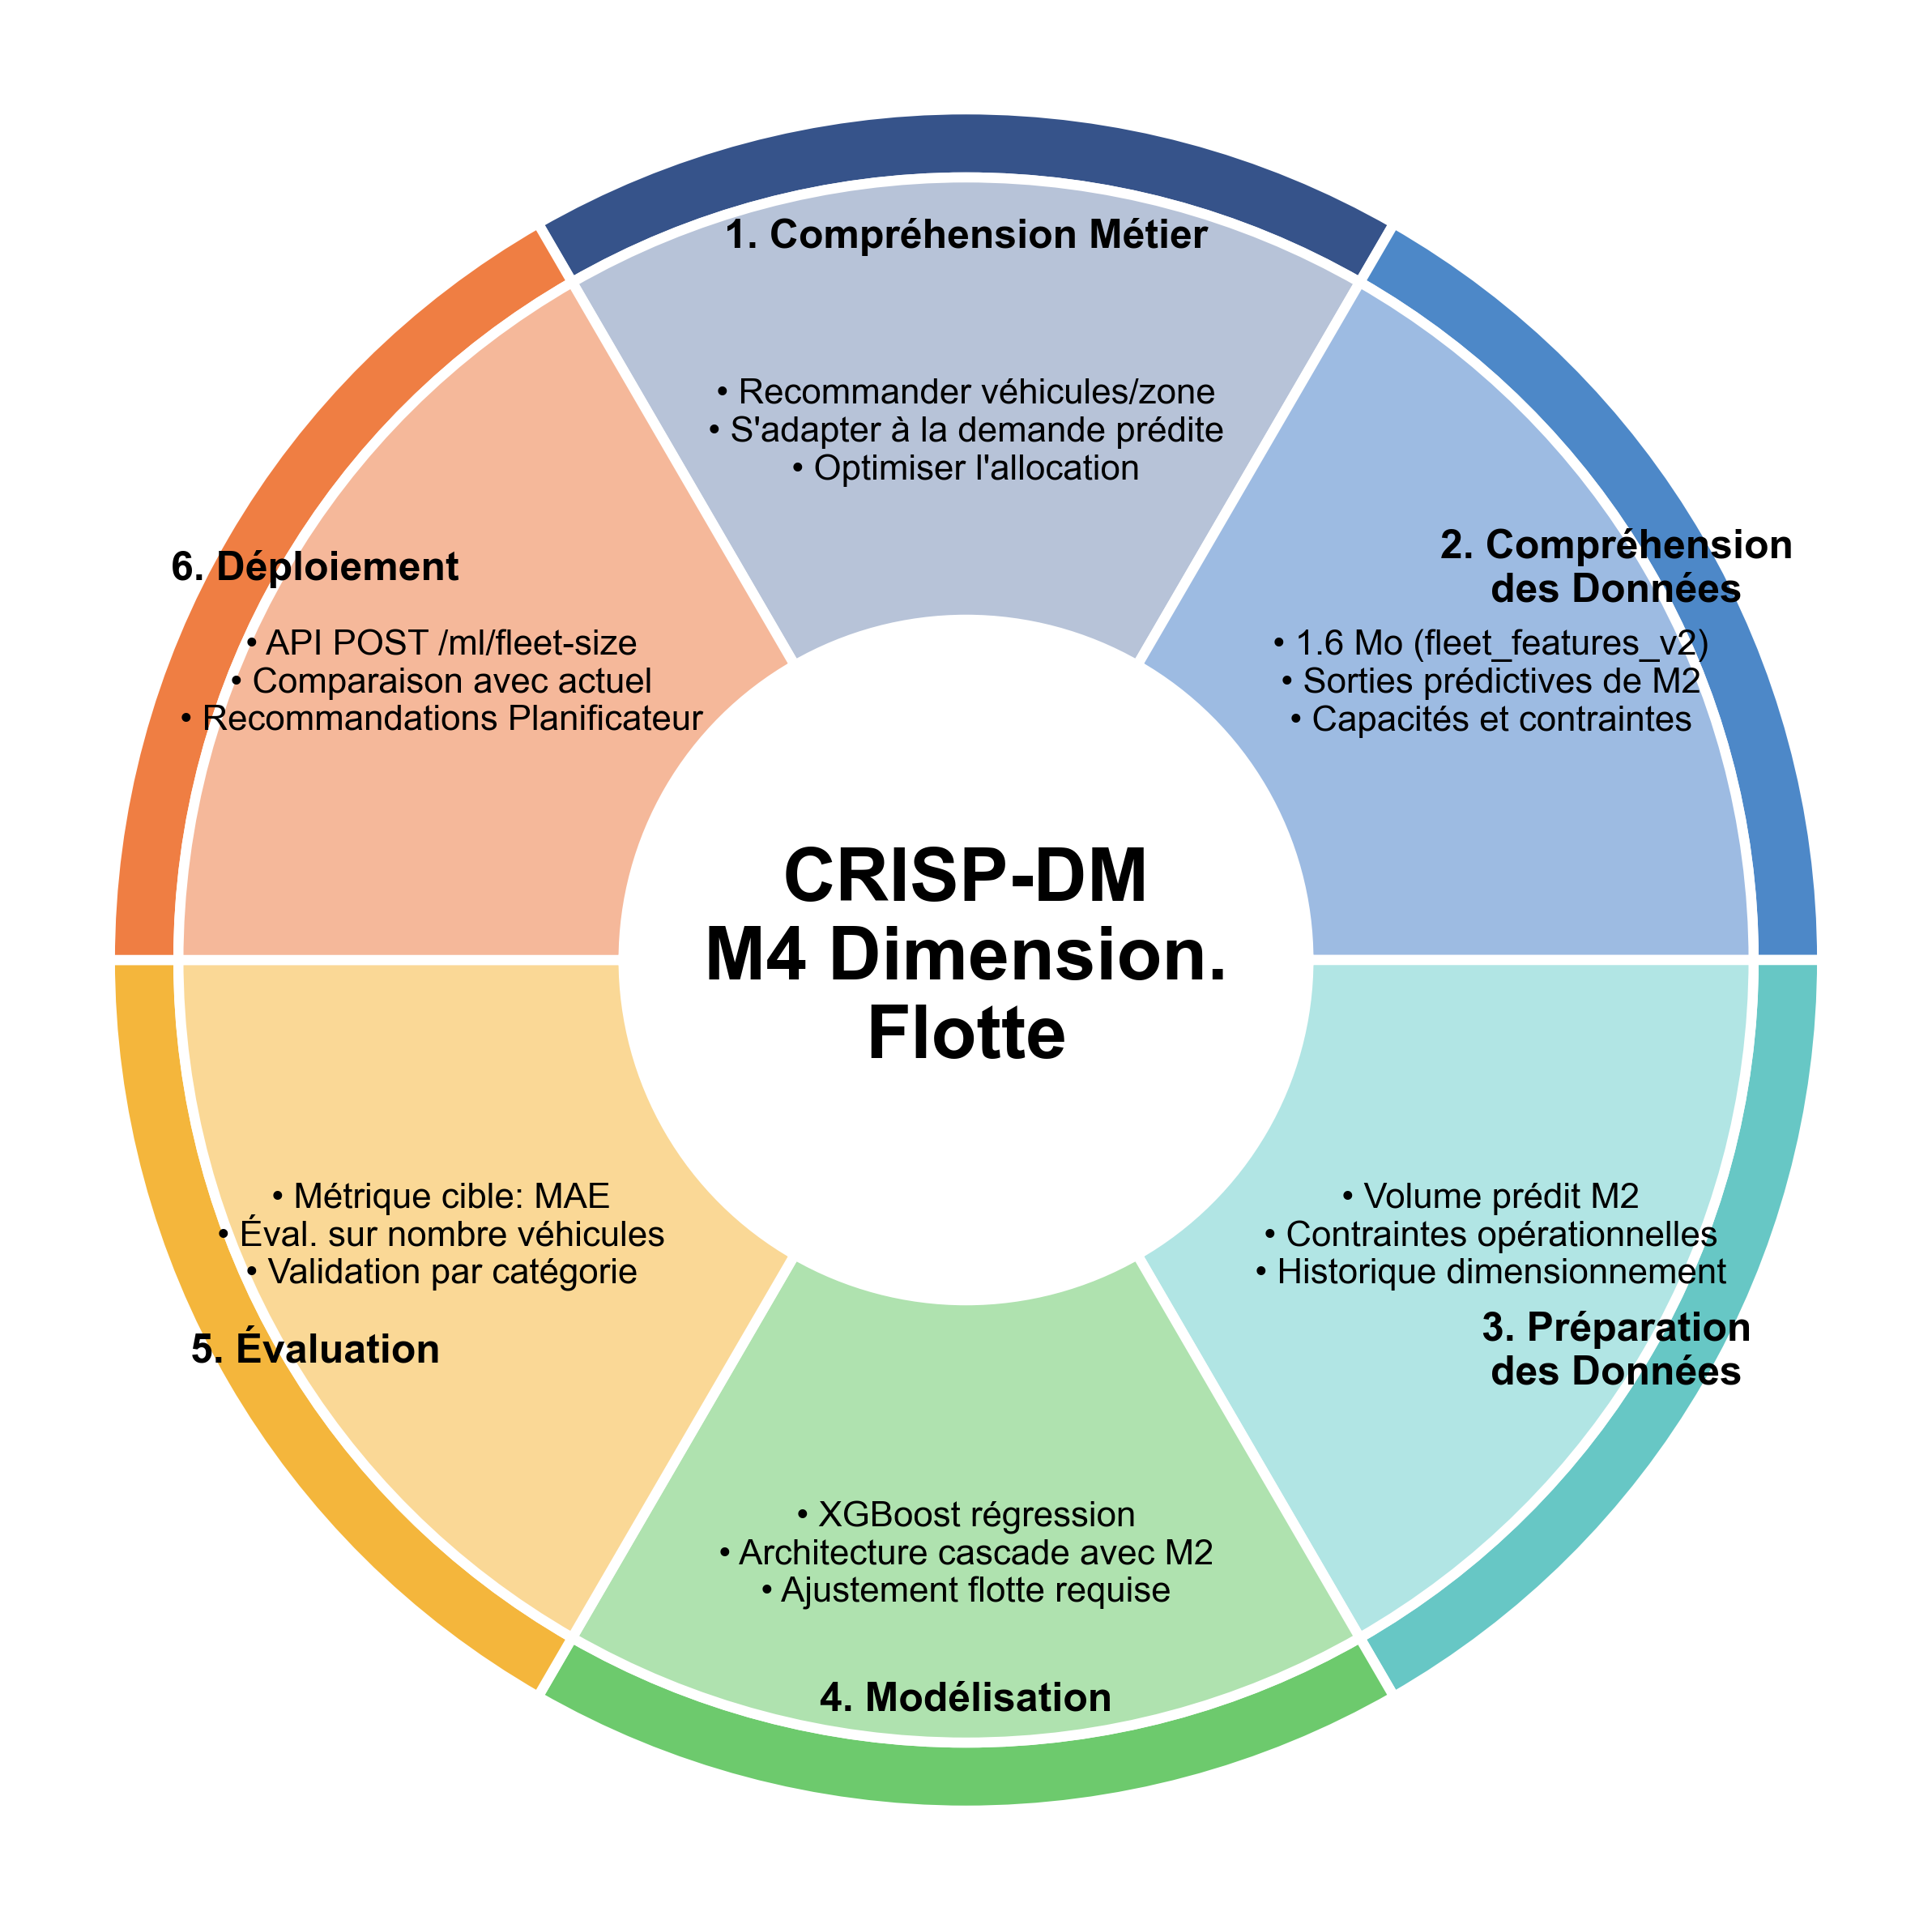
\includegraphics[width=0.88\linewidth]{img/crisp/crisp_dm_m4_fleet}
\caption{Diagramme CRISP-DM -- M4 Dimensionnement de Flotte}
\label{fig:crisp-m4}
\end{figure}

\begin{table}[H]
\centering
\setlength{\arrayrulewidth}{1pt}
\begin{tabular}{|p{3.5cm}|p{9.5cm}|}
\hline
\rowcolor{headerbg}
\multicolumn{2}{|c|}{\textbf{M4 -- Fleet Dimensioning}} \\
\hline
\textbf{Objectif métier} & Recommander le nombre optimal de véhicules par zone selon la demande prédite. \\
\hline
\textbf{Dataset} & \texttt{fleet\_features\_v2.parquet} (1,6~Mo) + sorties M2 (cascade). \\
\hline
\textbf{Features clés} & Volume prédit M2, capacité véhicule, contraintes opérationnelles, historique de dimensionnement. \\
\hline
\textbf{Algorithme} & XGBoost régression régularisée, architecture en cascade avec M2. \\
\hline
\textbf{Métrique cible} & MAE sur le nombre de véhicules recommandés. \\
\hline
\textbf{Intégration} & Recommandations de flotte dans le tableau de bord Planificateur avec comparaison flotte actuelle. \\
\hline
\end{tabular}
\caption{Fiche synthétique -- M4 Fleet Dimensioning}
\label{tab:m4-summary}
\end{table}
\setlength{\arrayrulewidth}{0.4pt}

\paragraph{Intégration dans l'application.}
Les recommandations de dimensionnement de flotte (nombre optimal de véhicules par zone) sont affichées dans le tableau de bord Planificateur avec une comparaison visuelle par rapport à la flotte actuelle.

\begin{figure}[H]
\centering
\IfFileExists{img/capture/ai/sp5_m4_fleet_sizing_composite.png}{%
  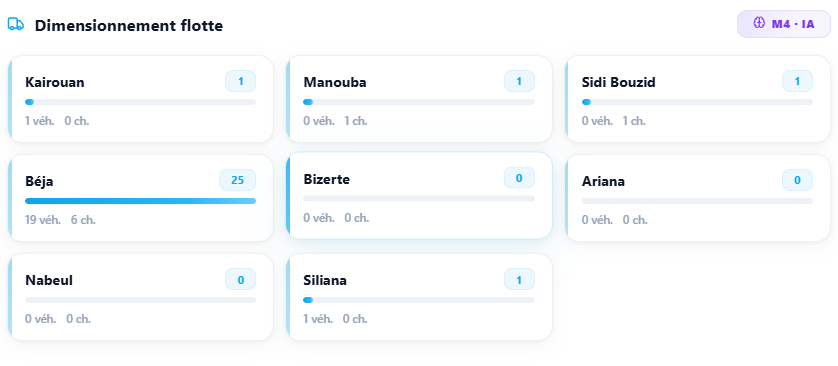
\includegraphics[width=\linewidth, keepaspectratio]{img/capture/ai/sp5_m4_fleet_sizing_composite}%
}{%
  \fbox{\parbox{0.9\linewidth}{\centering\vspace{4cm}\textit{[\`{}img/sp5\_m4\_fleet\_sizing\_composite\`{} --- Capture à réaliser]}\vspace{4cm}}}%
}
\caption{Intégration M4 Fleet Dimensioning : recommandations de dimensionnement de flotte par zone, comparaison avec la flotte actuelle}
\label{fig:sp5-m4-integration}
\end{figure}

\subsubsection{M5 -- Route Learning}

\begin{figure}[H]
\centering
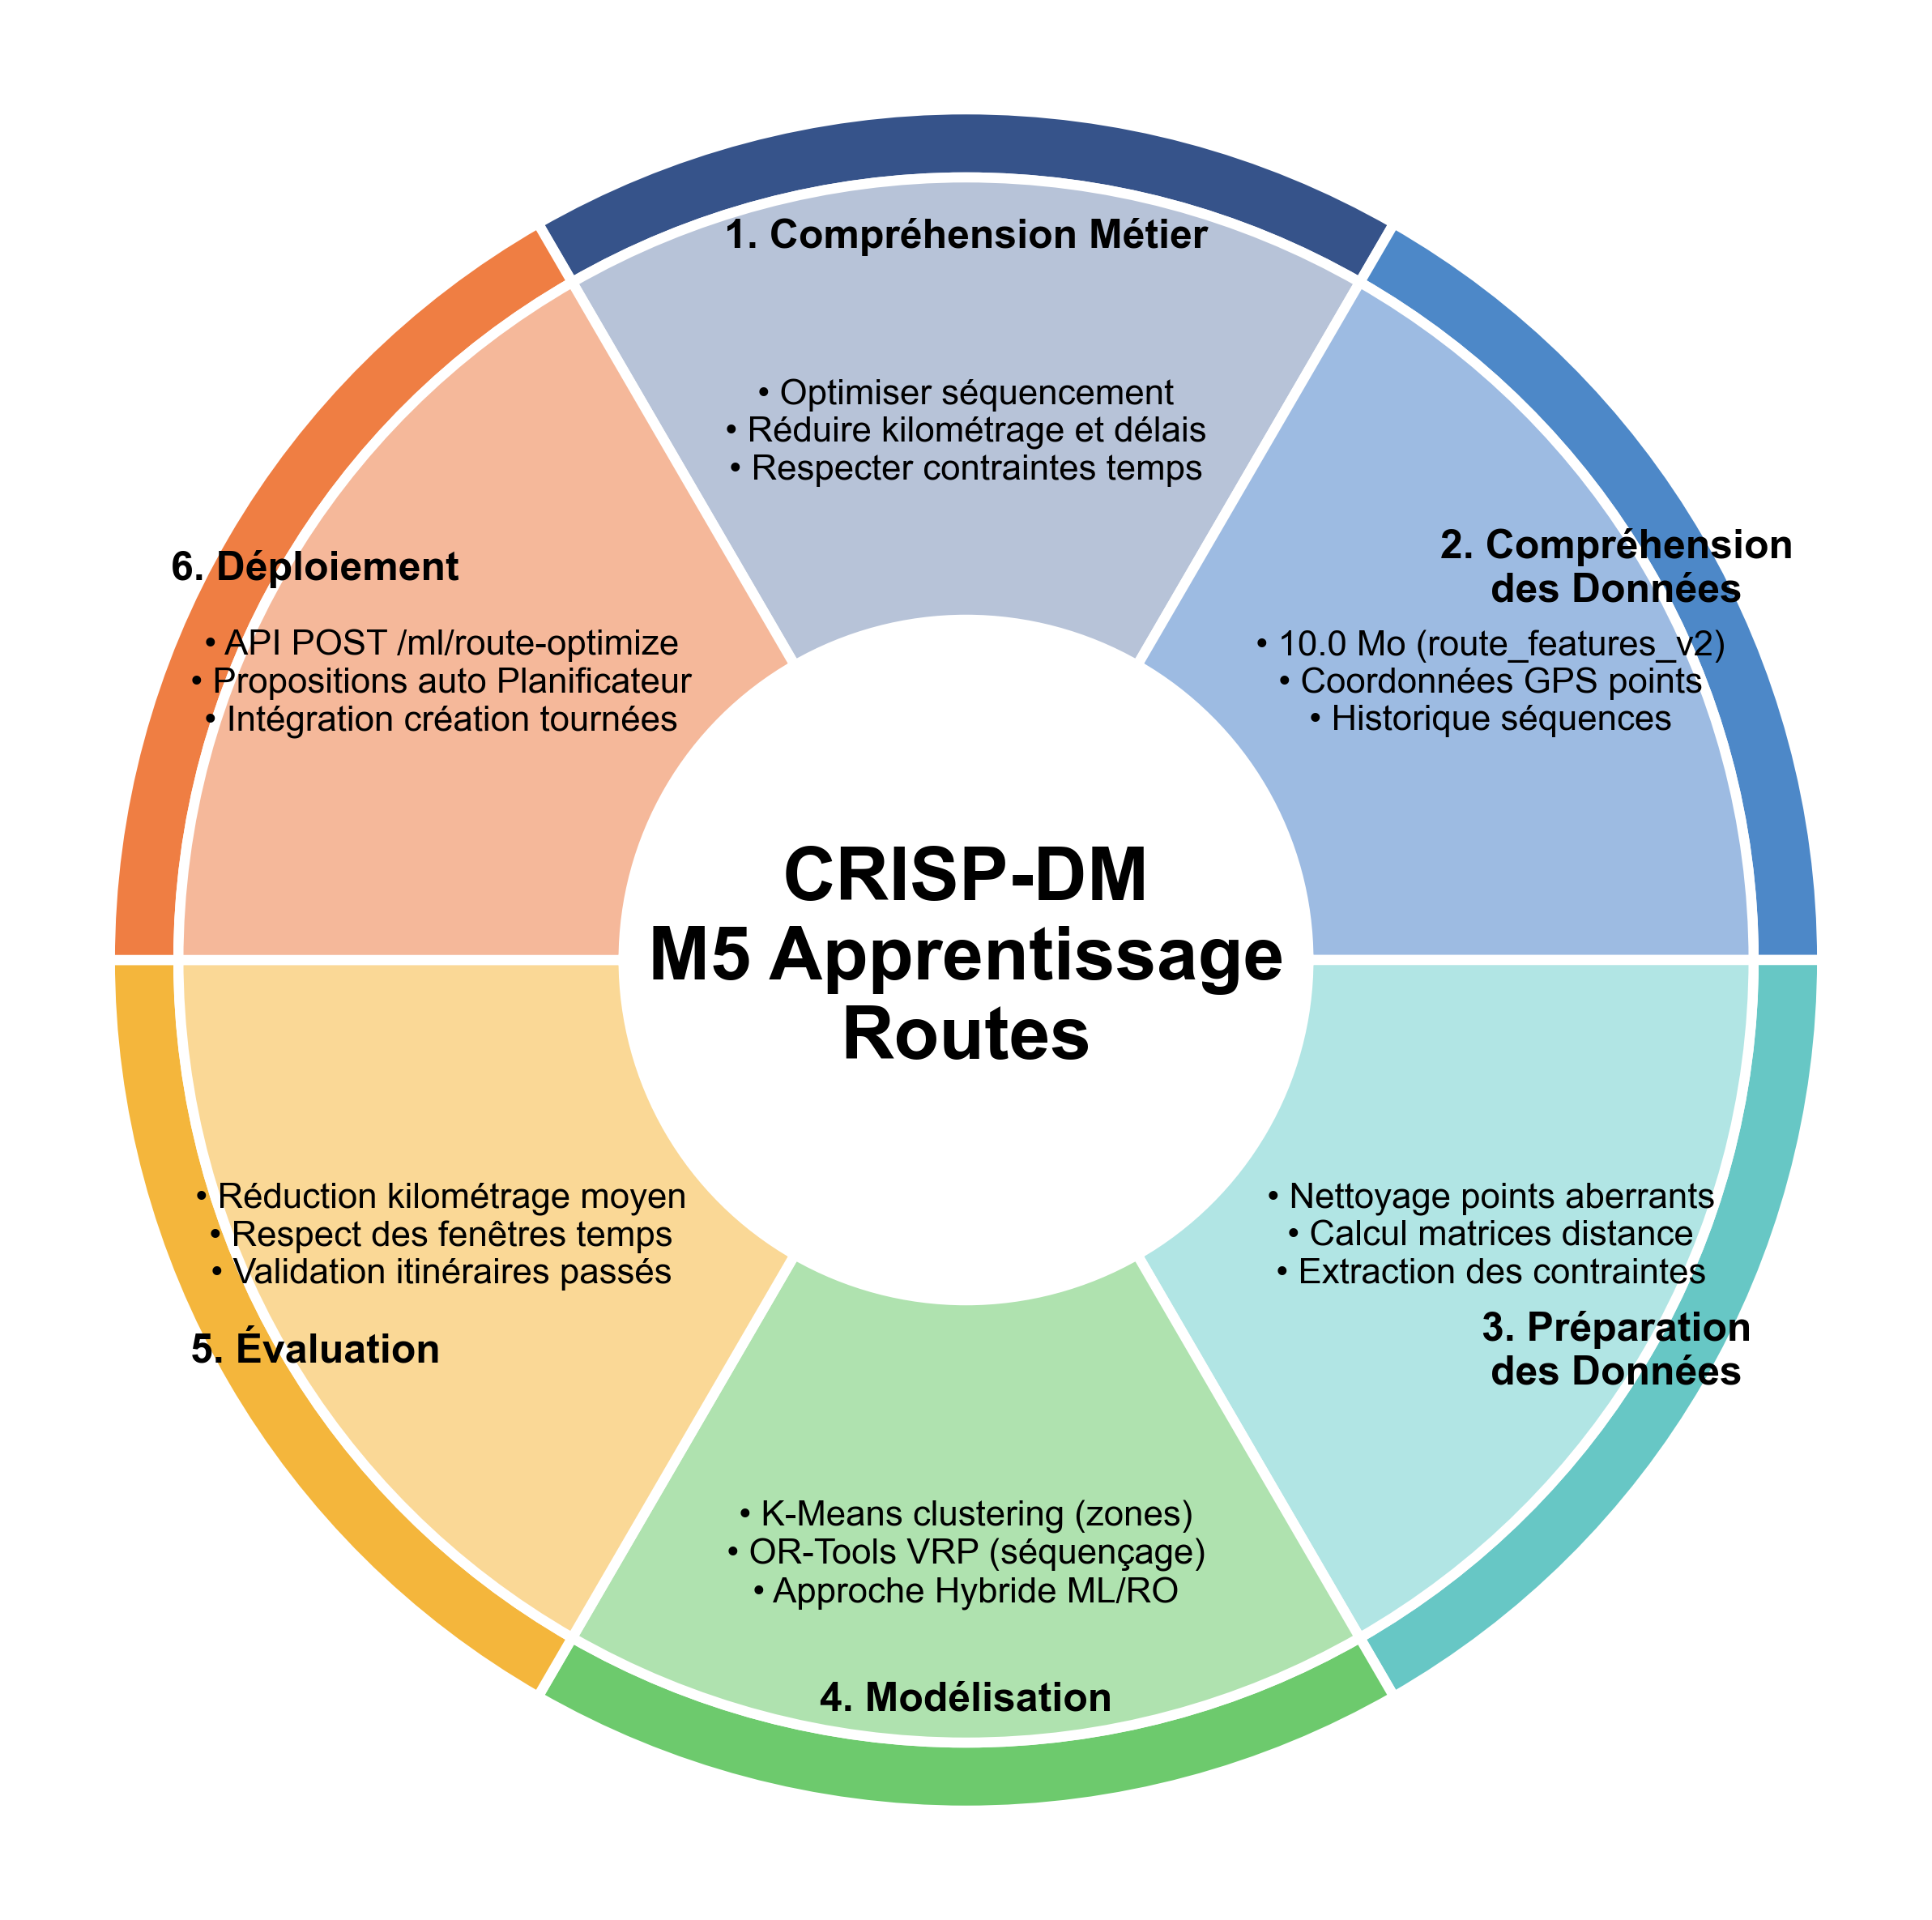
\includegraphics[width=0.88\linewidth]{img/crisp/crisp_dm_m5_route}
\caption{Diagramme CRISP-DM -- M5 Apprentissage des Routes}
\label{fig:crisp-m5}
\end{figure}

\begin{table}[H]
\centering
\setlength{\arrayrulewidth}{1pt}
\begin{tabular}{|p{3.5cm}|p{9.5cm}|}
\hline
\rowcolor{headerbg}
\multicolumn{2}{|c|}{\textbf{M5 -- Route Learning}} \\
\hline
\textbf{Objectif métier} & Optimiser le séquencement des tournées pour réduire le kilométrage et les délais. \\
\hline
\textbf{Dataset} & \texttt{route\_features\_v2.parquet} (10,0~Mo) \\
\hline
\textbf{Features clés} & Coordonnées GPS, historique de séquences efficaces, contraintes de temps, capacité. \\
\hline
\textbf{Algorithme} & Hybride : K-Means clustering (partitionnement de zones) + OR-Tools VRP (optimisation de séquence). \\
\hline
\textbf{Métrique cible} & Réduction du kilométrage moyen par tournée. \\
\hline
\textbf{Intégration} & Routes optimisées proposées au Planificateur lors de la création de tournées. \\
\hline
\end{tabular}
\caption{Fiche synthétique -- M5 Route Learning}
\label{tab:m5-summary}
\end{table}
\setlength{\arrayrulewidth}{0.4pt}

\paragraph{Modélisation et justification du modèle.}
Contrairement aux modèles prédictifs classiques (comme XGBoost utilisé pour le scoring), l'apprentissage des routes est un problème complexe d'optimisation combinatoire (VRP -- \textit{Vehicle Routing Problem}). Cinq approches algorithmiques ont été évaluées lors de cette phase. Les résultats obtenus sur un jeu de test de 500 tournées historiques sont présentés dans le tableau~\ref{tab:m5-evaluation}.

\begin{table}[H]
\centering
\setlength{\arrayrulewidth}{1pt}
\begin{tabular}{|l|c|c|p{4cm}|}
\hline
\rowcolor{headerbg}
\textbf{Algorithme} & \textbf{Écart à l'optimal (Gap)} & \textbf{Respect des délais} & \textbf{Temps d'exécution moyen} \\
\hline
Heuristique d'insertion & 14,5\,\% & 72\,\% & Très rapide (< 1 s) \\
\hline
Algorithme Génétique & 8,2\,\% & 84\,\% & Très lent ($\approx$ 5 min) \\
\hline
Recuit Simulé & 6,8\,\% & 87\,\% & Lent ($\approx$ 3 min) \\
\hline
OptaPlanner (Tabu Search) & 3,4\,\% & 94\,\% & Moyen ($\approx$ 1 min) \\
\hline
\textbf{K-Means + OR-Tools} & \textbf{1,2\,\%} & \textbf{98\,\%} & \textbf{Rapide ($\approx$ 10 s)} \\
\hline
\end{tabular}
\caption{Comparatif des algorithmes évalués pour le modèle M5 (Optimisation VRP)}
\label{tab:m5-evaluation}
\end{table}
\setlength{\arrayrulewidth}{0.4pt}

L'approche hybride \textbf{K-Means + OR-Tools} a été retenue. En premier lieu, l'algorithme K-Means pré-partitionne géographiquement les points de livraison (Clustering spatial), ce qui réduit drastiquement l'espace de recherche. Ensuite, le solveur OR-Tools de Google applique des heuristiques de routage avancées (\textit{Guided Local Search}) sur chaque cluster. En plus de garantir le meilleur respect des contraintes de temps (98\,\%), cette combinaison offre le compromis idéal entre la qualité de la solution (écart minimal de 1,2\,\%) et un temps d'exécution très court (10 secondes), une exigence fondamentale pour les planificateurs de PGH.

\paragraph{Intégration dans l'application.}
Les routes optimisées par M5 sont proposées au Planificateur sous forme de suggestions d'itinéraires dans l'interface de planification. Le Planificateur peut accepter, modifier ou rejeter chaque suggestion avec traitement de la rétroaction (\texttt{SuggestionIA.decision}).

\begin{figure}[H]
\centering
\IfFileExists{img/capture/ai/sp5_m5_route_suggestions_composite.png}{%
  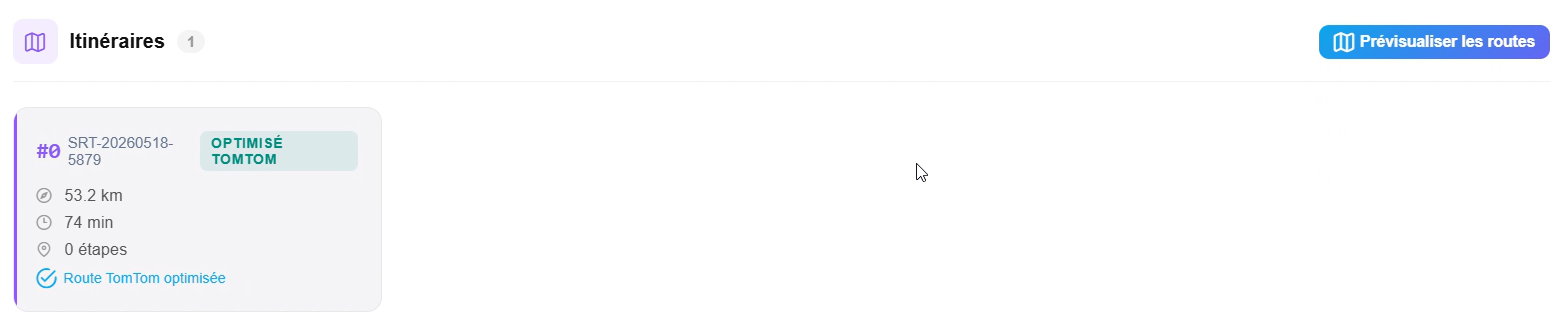
\includegraphics[width=\linewidth, keepaspectratio]{img/capture/ai/sp5_m5_route_suggestions_composite}%
}{%
  \fbox{\parbox{0.9\linewidth}{\centering\vspace{4cm}\textit{[\`{}img/sp5\_m5\_route\_suggestions\_composite\`{} --- Capture à réaliser]}\vspace{4cm}}}%
}
\caption{Intégration M5 Route Learning : interface suggestions d'itinéraires optimisés (K-Means + OR-Tools), score de qualité et actions Accepter / Modifier / Rejeter}
\label{fig:sp5-m5-integration}
\end{figure}

\subsubsection{M6 -- Payment Risk}

\begin{figure}[H]
\centering
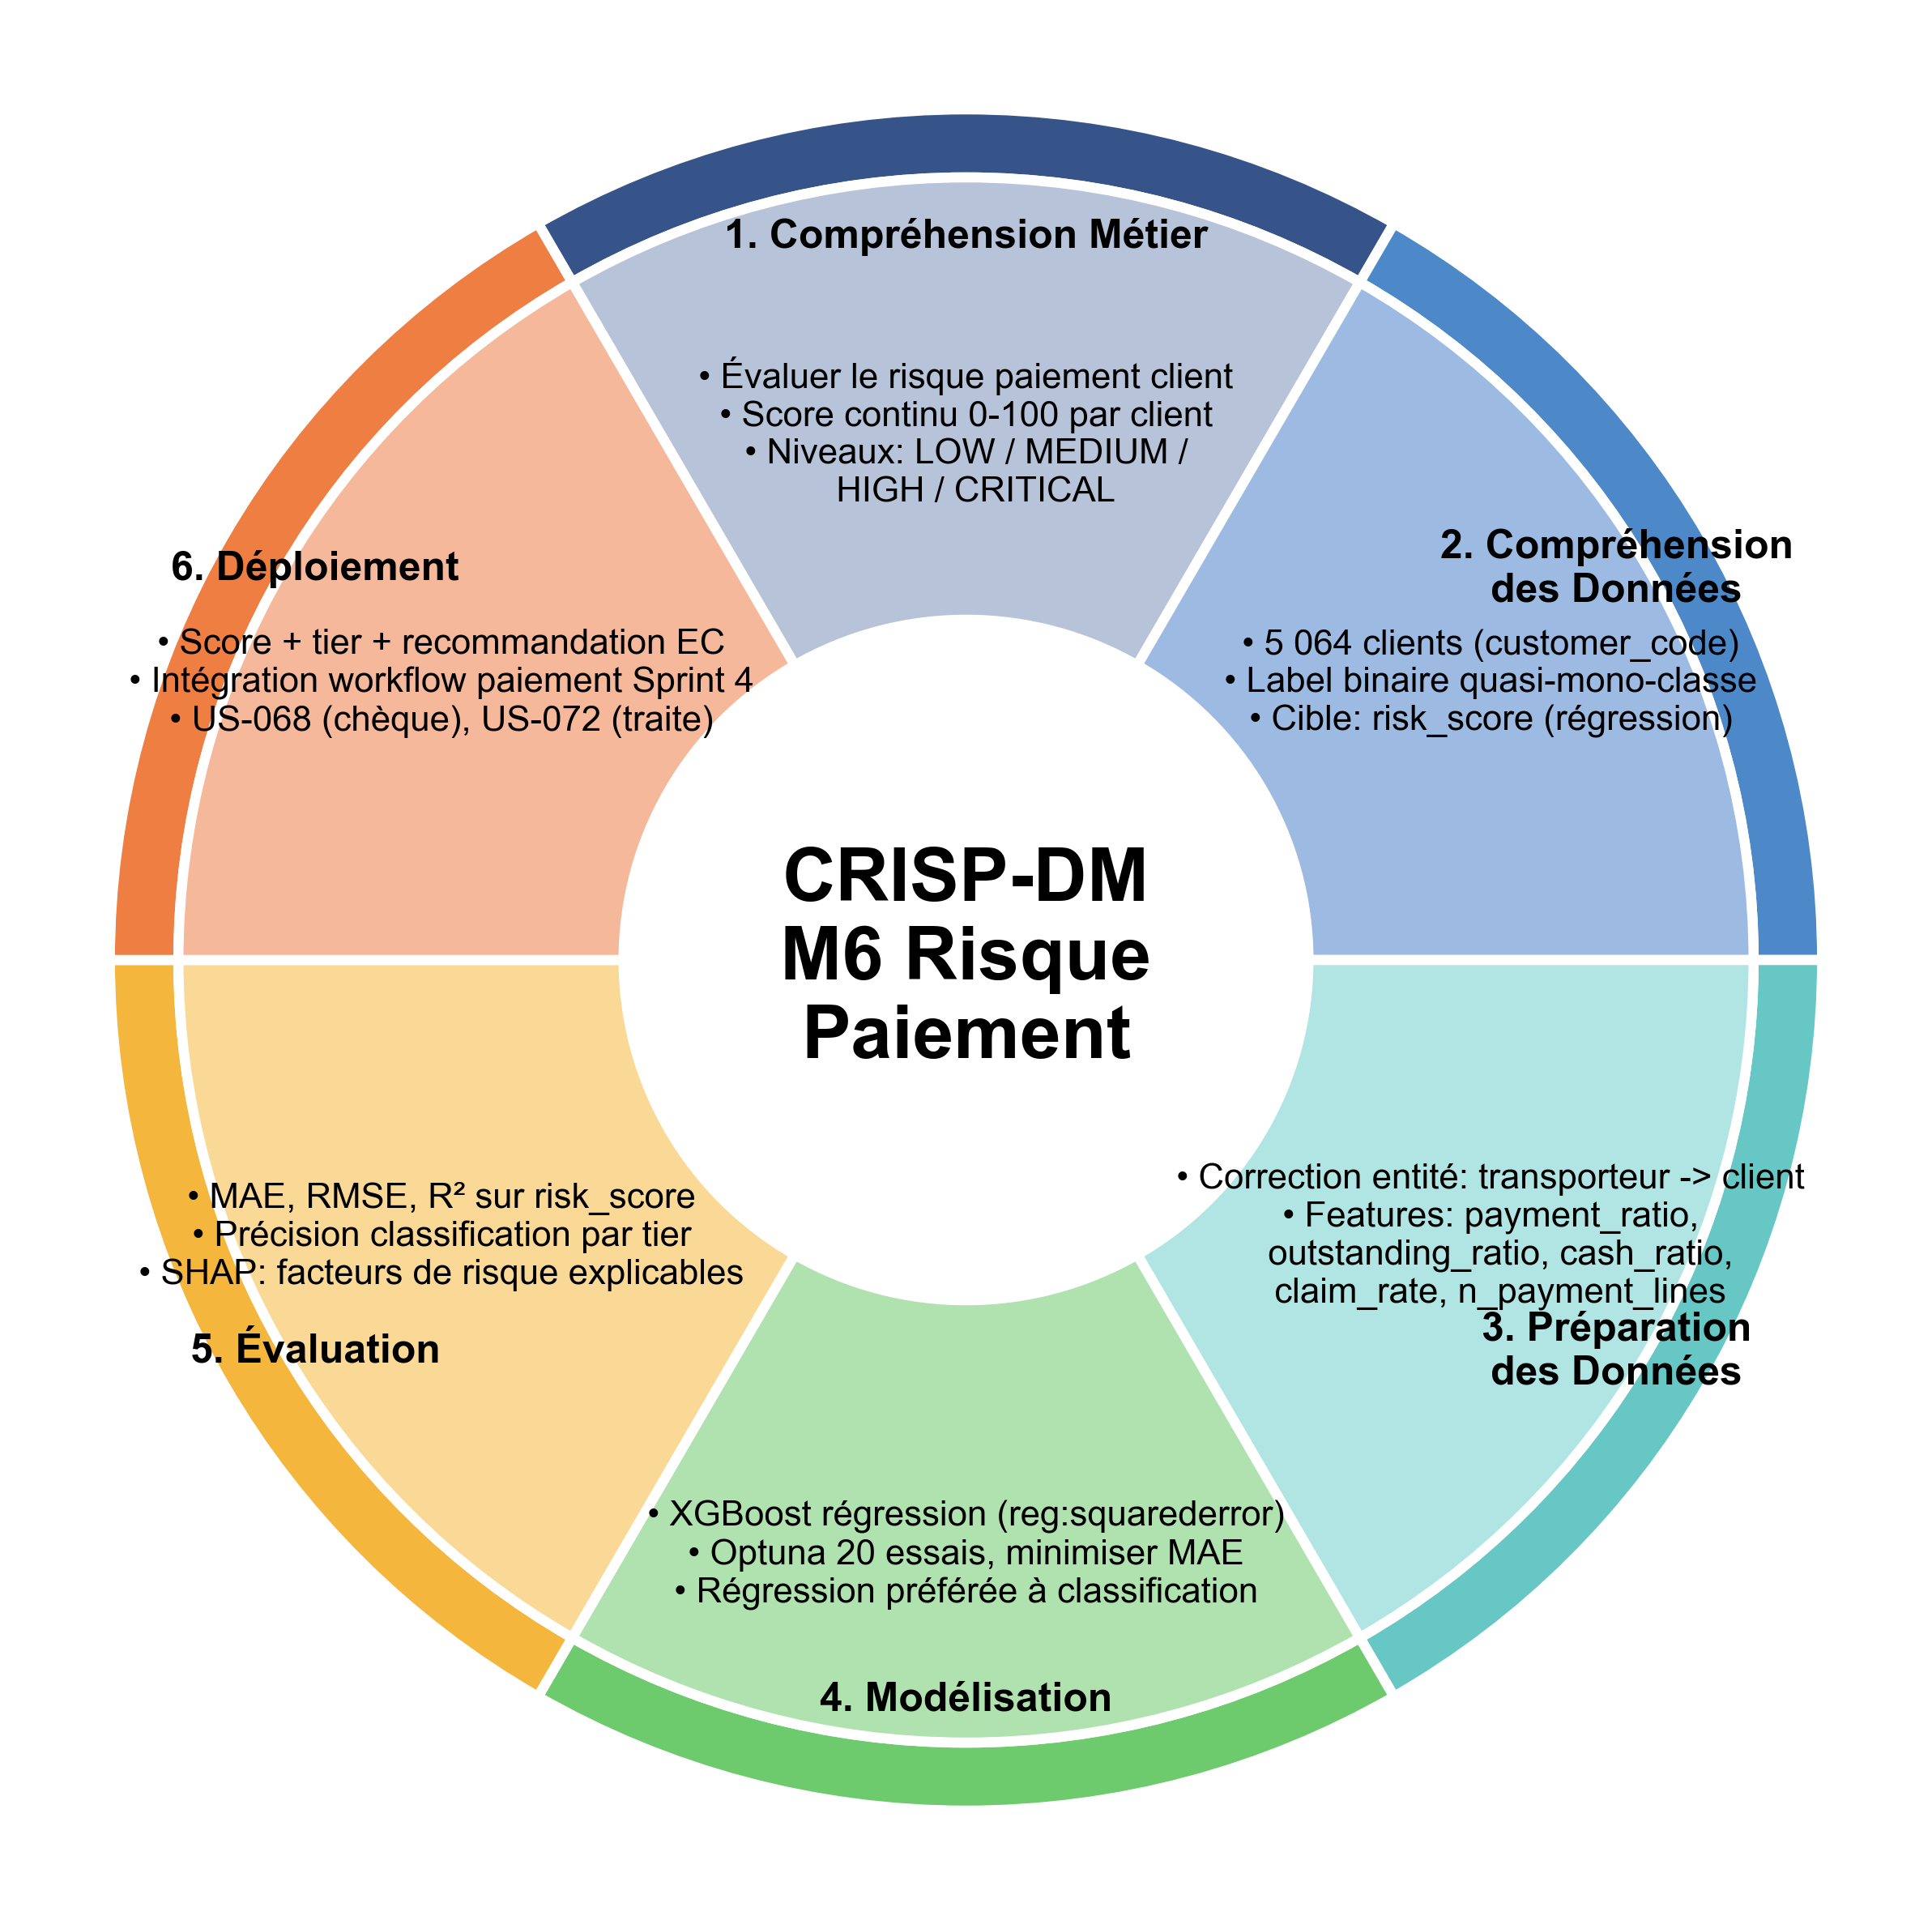
\includegraphics[width=0.88\linewidth]{img/crisp/crisp_dm_m6_payment}
\caption{Diagramme CRISP-DM -- M6 Risque Paiement Client}
\label{fig:crisp-m6}
\end{figure}

\begin{table}[H]
\centering
\setlength{\arrayrulewidth}{1pt}
\begin{tabular}{|p{3.5cm}|p{9.5cm}|}
\hline
\rowcolor{headerbg}
\multicolumn{2}{|c|}{\textbf{M6 -- Payment Risk}} \\
\hline
\textbf{Objectif métier} & Évaluer la solvabilité opérationnelle d'un client pour décider du mode de paiement autorisé. \\
\hline
\textbf{Dataset} & \texttt{payment\_risk\_v2.parquet} (0,3~Mo) \\
\hline
\textbf{Features clés} & Historique de paiements, taux d'incidents, ancienneté client, volume de commandes, délais de règlement. \\
\hline
\textbf{Algorithme} & XGBoost régression, score normalisé 0--100, seuils : Low / Medium / High / Critical. \\
\hline
\textbf{Métrique cible} & Corrélation entre score prédit et incidents de paiement réels. \\
\hline
\textbf{Intégration} & Score de risque visible par le REC lors de la validation d'une commande ou d'un paiement par traite. \\
\hline
\end{tabular}
\caption{Fiche synthétique -- M6 Payment Risk}
\label{tab:m6-summary}
\end{table}
\setlength{\arrayrulewidth}{0.4pt}

\paragraph{Intégration dans l'application.}
Le score de risque paiement (Low~/ Medium~/ High~/ Critical) est affiché par le REC lors de la validation d'une commande ou d'un paiement par traite, permettant une décision d'octroi de crédit informatisée.

\begin{figure}[H]
\centering
\IfFileExists{img/capture/ai/sp5_m6_payment_risk_composite.png}{%
  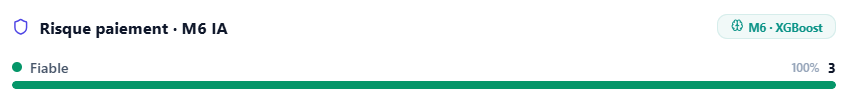
\includegraphics[width=\linewidth, keepaspectratio]{img/capture/ai/sp5_m6_payment_risk_composite}%
}{%
  \fbox{\parbox{0.9\linewidth}{\centering\vspace{4cm}\textit{[\`{}img/sp5\_m6\_payment\_risk\_composite\`{} --- Capture à réaliser]}\vspace{4cm}}}%
}
\caption{Intégration M6 Payment Risk : score de risque paiement (Low / Medium / High / Critical) affiché au REC lors de la validation d'une commande}
\label{fig:sp5-m6-integration}
\end{figure}

\subsubsection{Tableau comparatif des six modèles}

\begin{table}[H]
\centering
\setlength{\arrayrulewidth}{1pt}
\resizebox{\textwidth}{!}{%
\begin{tabular}{|l|l|l|l|l|}
\hline
\rowcolor{headerbg}
\textbf{Modèle} & \textbf{Type} & \textbf{Algorithme} & \textbf{Métrique} & \textbf{Endpoint FastAPI} \\
\hline
M1 Driver Scoring & Classification & XGBoost & F1 / AUC-ROC & \texttt{/ml/driver-score} \\
\hline
M2 Demand Forecast & Régression multi & XGBoost & MAPE $<$15\,\% & \texttt{/ml/demand-forecast} \\
\hline
M3 Delay Prediction & Classification & XGBoost & PR-AUC & \texttt{/ml/delay-risk} \\
\hline
M4 Fleet Sizing & Régression & XGBoost (cascade) & MAE & \texttt{/ml/fleet-size} \\
\hline
M5 Route Learning & Clustering + VRP & K-Means + OR-Tools & km réduit & \texttt{/ml/route-optimize} \\
\hline
M6 Payment Risk & Régression & XGBoost & Score 0--100 & \texttt{/ml/payment-risk} \\
\hline
\end{tabular}%
}
\caption{Comparatif des six modèles ML déployés dans Fleet~AI}
\label{tab:ml-comparatif}
\end{table}
\setlength{\arrayrulewidth}{0.4pt}

% -----------------------------------------------------------
\subsection{Architecture LLM et Chatbot Text-to-SQL}
% -----------------------------------------------------------

Fleet~AI intègre un chatbot analytique fondé sur le modèle \textbf{Gemma~4 31B} déployé localement via \textbf{Ollama}. L'utilisateur interroge la base de données en langage naturel ; le système génère, valide et exécute la requête SQL correspondante, puis reformule le résultat en texte. Ce déploiement on-premise est une contrainte métier : PGH ne peut pas externaliser ses données opérationnelles vers des API cloud tierces.

\subsubsection{Architecture globale}

% ============================================================
% FIGURE 8.8 — Architecture Text-to-SQL locale
% ============================================================
%
%  Layout (3 couches horizontales, pipeline en Z) :
%
%  ┌─────────────────────────── Frontend ──────────────────────┐
%  │  [Utilisateur]                                            │
%  └───────────────────────────────────────────────────────────┘
%  ┌─────────────────────────── Backend ───────────────────────┐
%  │  (1)Auth → (2)Session → (3)Intention → (4)Génération SQL  │
%  │                                              ↓            │
%  │  (7)Reformulation ← (6)Exécution ← (5)Validation         │
%  └───────────────────────────────────────────────────────────┘
%  ┌──────────────────── Infrastructure On-Premise ────────────┐
%  │  Redis/MongoDB     Ollama LLM      PostgreSQL  Schéma.md  │
%  └───────────────────────────────────────────────────────────┘
%
%  Règles de routage sans croisement :
%  • Pipeline principal : flèches bleues horizontales dans chaque rangée
%  • Retour (7)→Utilisateur : monte à gauche via couloir x=2.0
%  • Dépendances infra : flèches verticales directes
%    chaque nœud backend est aligné verticalement avec son infra
%
% ============================================================
% FIGURE 8.8 — Architecture Text-to-SQL locale
% ============================================================
\begin{figure}[H]
\centering
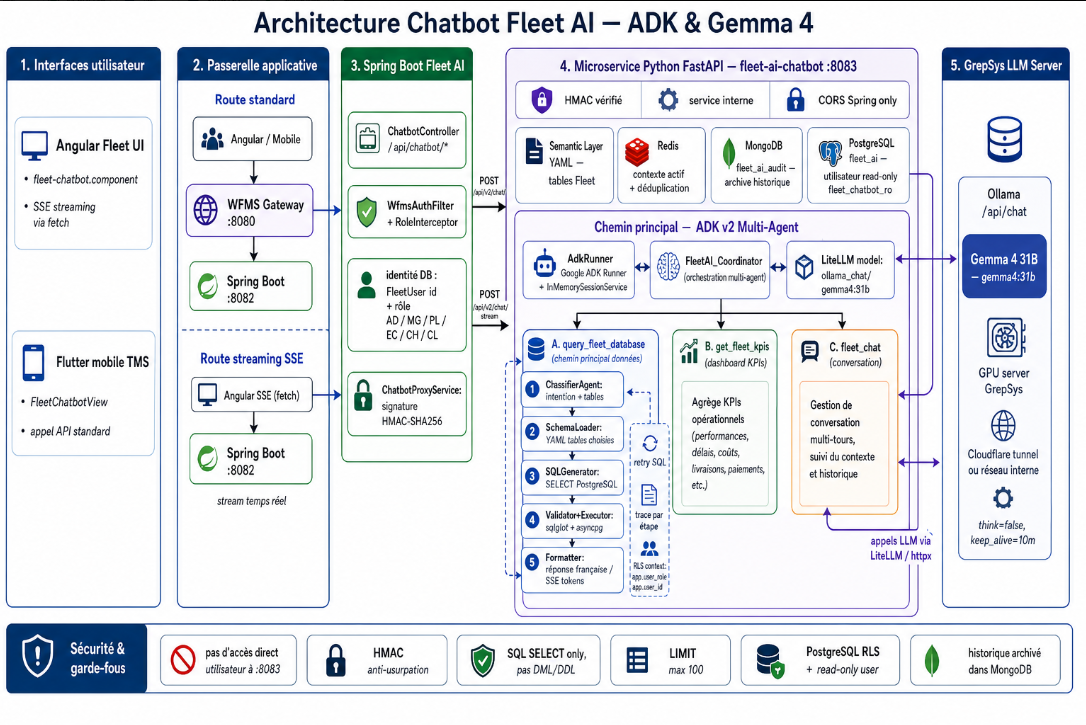
\includegraphics[width=\linewidth, keepaspectratio]{img/figure/chatBot}
\caption{Architecture Text-to-SQL locale --- Pipeline 7 étapes du Chatbot Fleet~AI (Gemma~4 31B via Ollama, déploiement on-premise PGH)}
\label{fig:dfd-chatbot}
\end{figure}


\subsubsection{Pipeline conversationnel}

Le traitement d'une requête utilisateur suit sept étapes :

\begin{enumerate}
  \item \textbf{Authentification et contexte} : la requête est reçue par le backend Spring Boot. L'identité et le rôle de l'utilisateur (RBAC) déterminent le périmètre de données accessible.
  \item \textbf{Gestion de session} : l'historique conversationnel est stocké dans \textbf{Redis} (TTL~30~min) pour maintenir le contexte entre les échanges successifs. Les conversations sont archivées dans \textbf{MongoDB}.
  \item \textbf{Compréhension de l'intention} : Gemma~4 31B analyse la question et identifie l'intention métier (reporting, agrégation, filtrage, tendance).
  \item \textbf{Génération SQL} : le LLM génère une requête SQL guidée par un \textit{schema prompt} injectant la structure relationnelle de Fleet~AI (tables, colonnes, relations).
  \item \textbf{Validation et sécurité} : un validateur intercepte la requête avant exécution -- blocage des instructions d'écriture (\texttt{INSERT}, \texttt{UPDATE}, \texttt{DELETE}), vérification syntaxique, contrôle des tables autorisées selon le rôle (RLS).
  \item \textbf{Exécution} : la requête validée s'exécute en lecture seule sur PostgreSQL.
  \item \textbf{Reformulation} : le jeu de résultats est retourné à Gemma~4 31B qui produit une réponse textuelle structurée, accessible depuis le frontend Angular (web) ou Flutter (mobile).
\end{enumerate}

\subsubsection{Sécurité et contraintes techniques}

\begin{table}[H]
\centering
\setlength{\arrayrulewidth}{1pt}
\begin{tabular}{|p{4cm}|p{9.5cm}|}
\hline
\rowcolor{headerbg}
\textbf{Composant} & \textbf{Rôle dans le pipeline} \\
\hline
Ollama & Serveur d'inférence local pour Gemma~4 31B. Aucune donnée ne quitte l'infrastructure PGH. \\
\hline
Redis & Cache de session conversationnelle (TTL configurable, éviction LRU). \\
\hline
MongoDB & Archivage persistant des conversations pour audit et ré-entraînement futur. \\
\hline
SQL Validator & Middleware Spring Boot : whitelist de tables, blocage DDL/DML, contrôle de la profondeur des jointures. \\
\hline
RLS (Row-Level Security) & Restriction PostgreSQL : chaque rôle ne voit que les données de son périmètre (zone, entreprise, tournée). \\
\hline
Spring Boot & Point d'entrée REST sécurisé (JWT), orchestrateur du pipeline multi-étapes. \\
\hline
\end{tabular}
\caption{Composants de l'architecture chatbot Text-to-SQL}
\label{tab:chatbot-components}
\end{table}
\setlength{\arrayrulewidth}{0.4pt}

\paragraph{Intégration dans l'application.}
L'interface de chatbot est accessible depuis le tableau de bord Manager (Angular) et depuis l'application mobile Flutter. L'utilisateur pose une question en français ou en arabe ; la réponse est affichée sous forme textuelle avec un tableau de données lorsque la question porte sur des agrégations ou des classements.

\begin{figure}[H]
\centering
\IfFileExists{img/capture/ai/sp5_chatbot_composite.png}{%
  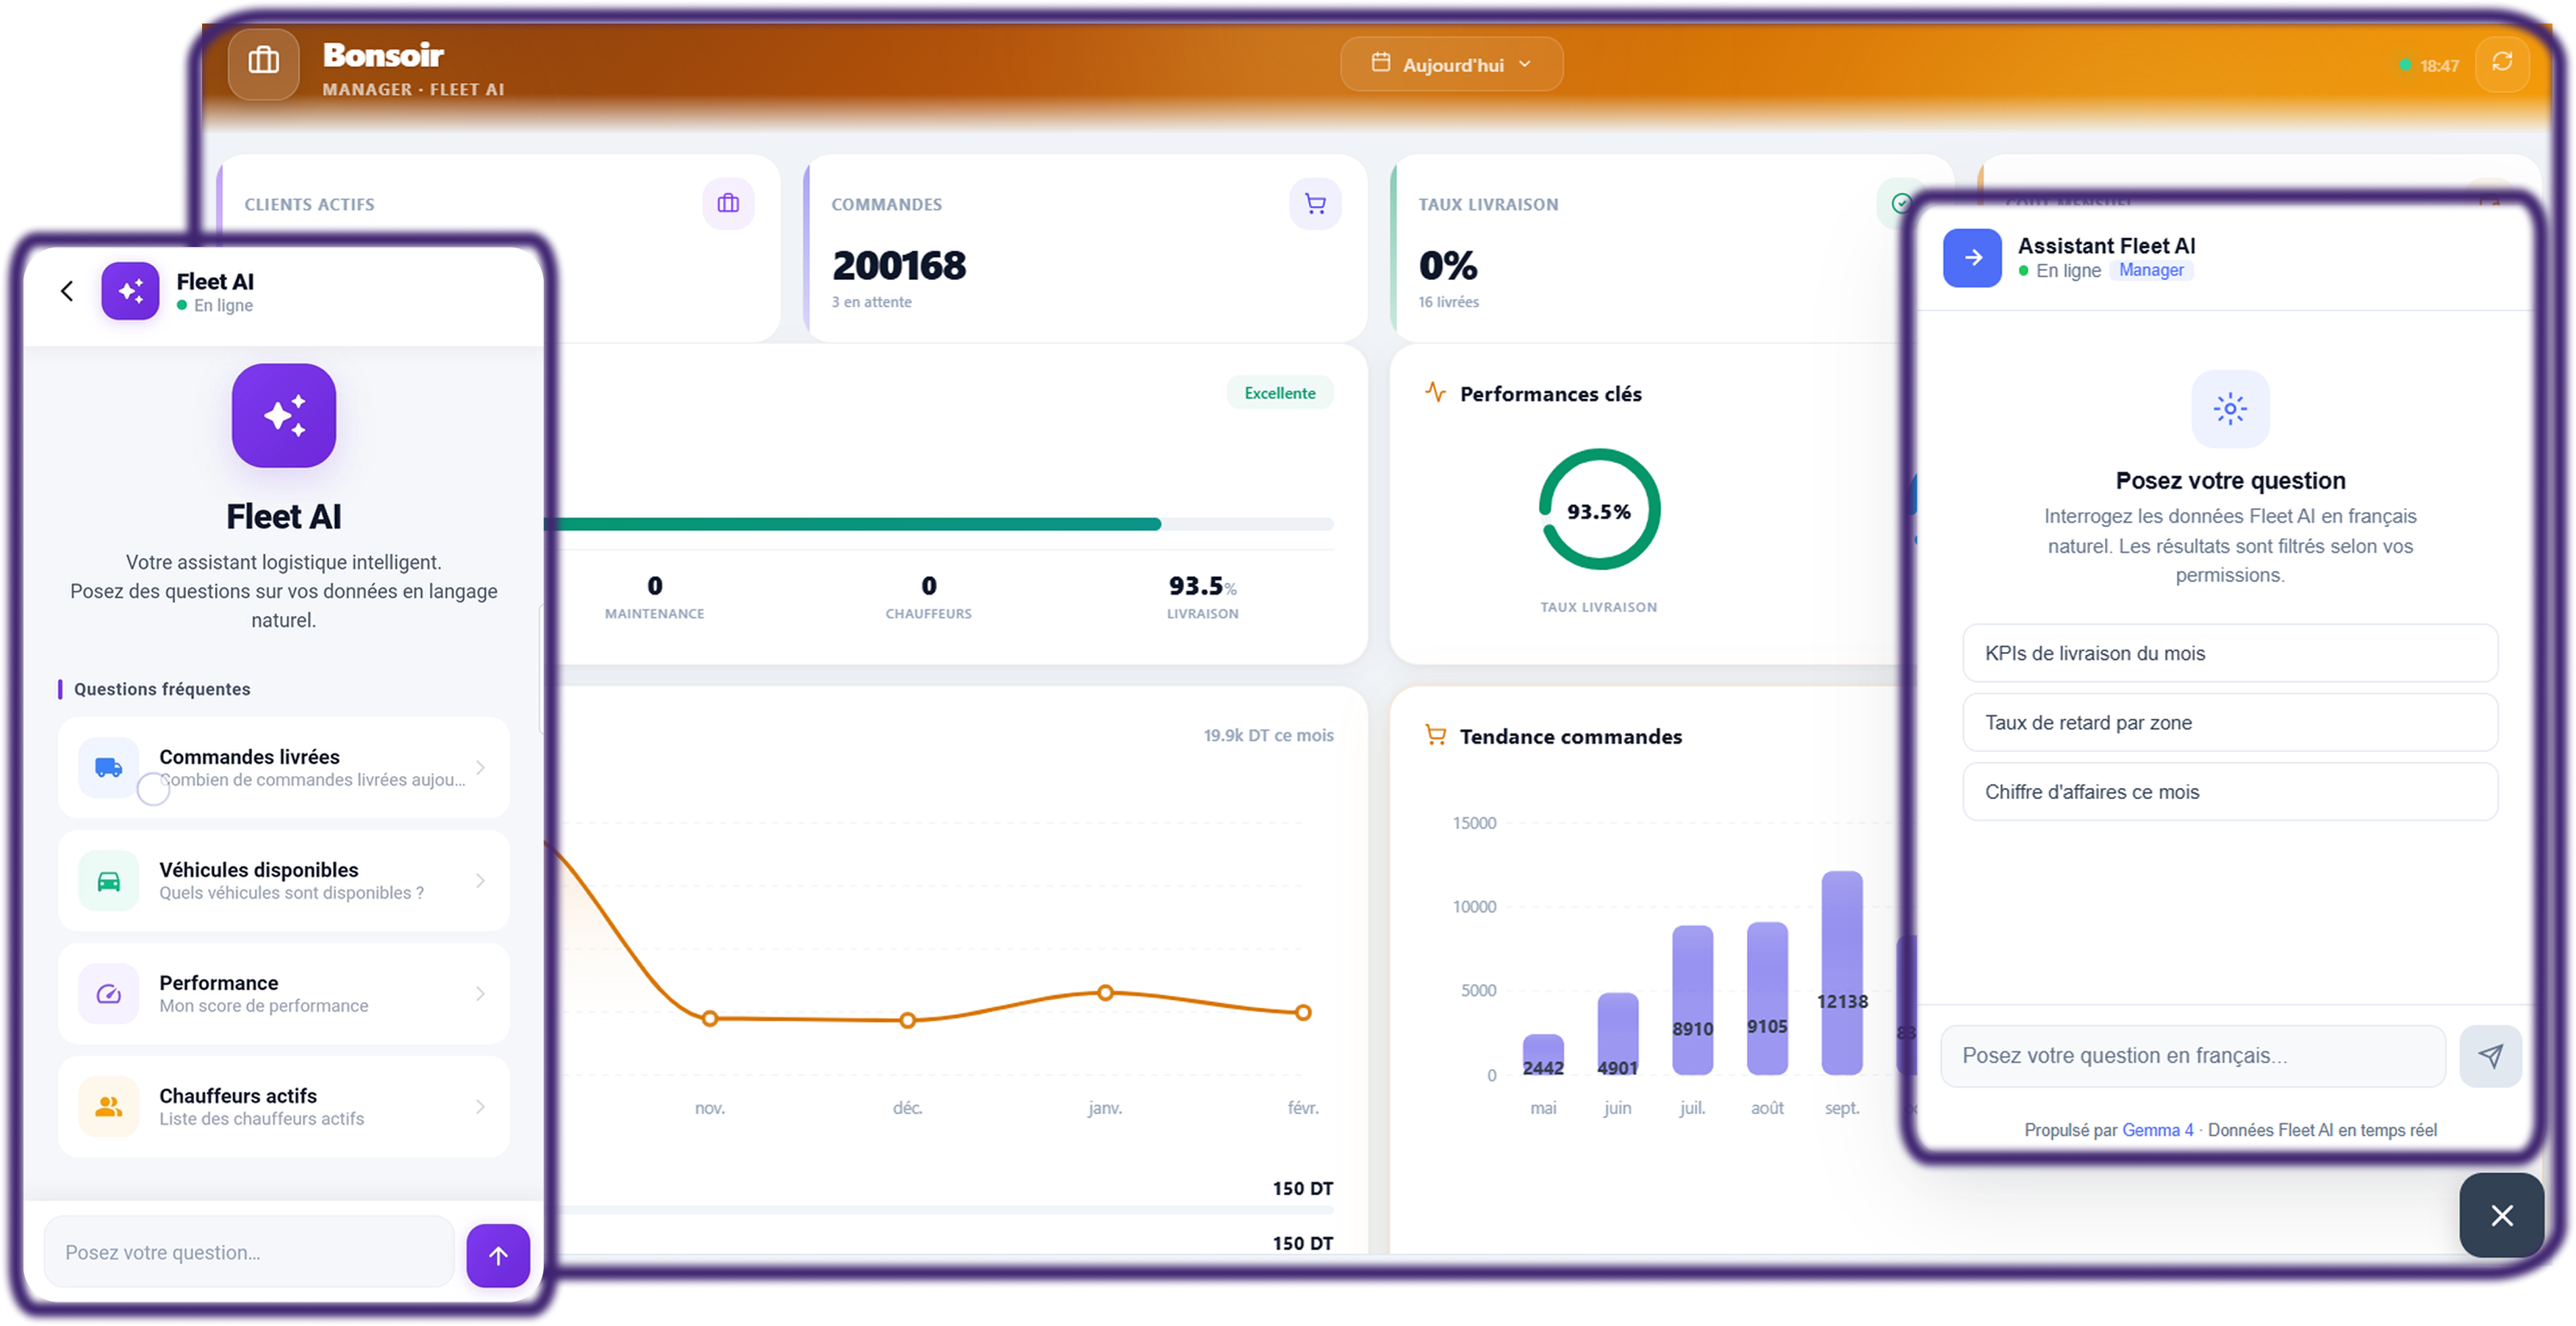
\includegraphics[width=\linewidth, keepaspectratio]{img/capture/ai/sp5_chatbot_composite}%
}{%
  \fbox{\parbox{0.9\linewidth}{\centering\vspace{4cm}\textit{[\`{}img/sp5\_chatbot\_composite\`{} --- Capture à réaliser]}\vspace{4cm}}}%
}
\caption{Intégration Chatbot Text-to-SQL : interface conversationnelle en langage naturel, génération SQL automatique et réponse reformulée par Gemma~4 31B}
\label{fig:sp5-chatbot-integration}
\end{figure}



% =============================================================
\section{Tests}
% =============================================================

Afin de valider la robustesse de la couche IA déployée, des tests de charge ont été exécutés sur l'API d'Intelligence Artificielle à l'aide de \textbf{JMeter}, simulant des appels simultanés aux six modèles ML et au chatbot Text-to-SQL.

\begin{figure}[H]
\centering
\IfFileExists{img/capture/ai/sp5_test_jmeter.png}{%
  \includegraphics[width=\linewidth, keepaspectratio]{img/capture/ai/sp5_test_jmeter}%
}{%
  \fbox{\parbox{0.9\linewidth}{\centering\vspace{4cm}\textit{[img/capture/ai/sp5\_test\_jmeter.png]}\vspace{4cm}}}%
}
\caption{Exécution d'un test de charge avec JMeter sur l'API d'Intelligence Artificielle}
\label{fig:sp5-test-jmeter}
\end{figure}

\section*{Conclusion}
\addcontentsline{toc}{section}{Conclusion}

Le Sprint~5 achève Fleet~AI. Les six modèles ML (scoring chauffeur, prévision de la demande, détection des retards, dimensionnement de flotte, apprentissage des routes, risque paiement) sont déployés via FastAPI selon la méthodologie CRISP-DM. Le chatbot Text-to-SQL fondé sur Gemma~4 31B permet d'interroger la base de données en langage naturel.
